%%%%%%%%%%%%%%%%%%%%%%%%%%%%%%%%%%%%%%%%%%%%%%%%%%%%%%%%%%%%%%%%%%%%%%%%%%%%%%%
%                       CARREGA DE LA CLASSE DE DOCUMENT                      %
%                                                                             %
% Les opcions admissibles son:                                                %
%      12pt / 11pt            (cos dels tipus de lletra; no feu servir 10pt)  %
%                                                                             %
% catalan/spanish/english     (llengua principal del treball)                 %
%                                                                             % 
% french/italian/german...    (si necessiteu fer servir alguna altra llengua) %
%                                                                             %
% listoffigures               (El document inclou un Index de figures)        %
% listoftables                (El document inclou un Index de taules)         %
% listofquadres               (El document inclou un Index de quadres)        %
% listofalgorithms            (El document inclou un Index d'algorismes)      %
%                                                                             %
%%%%%%%%%%%%%%%%%%%%%%%%%%%%%%%%%%%%%%%%%%%%%%%%%%%%%%%%%%%%%%%%%%%%%%%%%%%%%%%

\documentclass[11pt,spanish,listoffigures]{tfgetsinf}

%%%%%%%%%%%%%%%%%%%%%%%%%%%%%%%%%%%%%%%%%%%%%%%%%%%%%%%%%%%%%%%%%%%%%%%%%%%%%%%
%                     CODIFICACIO DEL FITXER FONT                             %
%                                                                             %
%    windows fa servir normalment 'ansinew'                                   %
%    amb linux es possible que siga 'latin1' o 'latin9'                       %
%    Pero el mes recomanable es fer servir utf8 (unicode 8)                   %
%                                          (si el vostre editor ho permet)    % 
%%%%%%%%%%%%%%%%%%%%%%%%%%%%%%%%%%%%%%%%%%%%%%%%%%%%%%%%%%%%%%%%%%%%%%%%%%%%%%%

\usepackage[utf8]{inputenc} 
\usepackage{multirow}
\usepackage{babel}

\usepackage{natbib}
\bibliographystyle{plain}
\graphicspath{ {Imagenes/} }

%%%%%%%%%%%%%%%%%%%%%%%%%%%%%%%%%%%%%%%%%%%%%%%%%%%%%%%%%%%%%%%%%%%%%%%%%%%%%%%
%                        ALTRES PAQUETS I DEFINICIONS                         %
%                                                                             %
% Carregueu aci els paquets que necessiteu i declareu les comandes i entorns  %
%                                          (aquesta seccio pot ser buida)     %
%%%%%%%%%%%%%%%%%%%%%%%%%%%%%%%%%%%%%%%%%%%%%%%%%%%%%%%%%%%%%%%%%%%%%%%%%%%%%%%



%%%%%%%%%%%%%%%%%%%%%%%%%%%%%%%%%%%%%%%%%%%%%%%%%%%%%%%%%%%%%%%%%%%%%%%%%%%%%%%
%                        DADES DEL TREBALL                                    %
%                                                                             %
% titol, alumne, tutor i curs academic                                        %
%%%%%%%%%%%%%%%%%%%%%%%%%%%%%%%%%%%%%%%%%%%%%%%%%%%%%%%%%%%%%%%%%%%%%%%%%%%%%%%

\title{ Desarrollo de software basado en microservicios: un caso de estudio para evaluar sus ventajas e inconvenientes }
\author{Víctor Alberto Iranzo Jiménez}
\tutor{Patricio Orlando Letelier Torres}
\curs{2017-2018}

%%%%%%%%%%%%%%%%%%%%%%%%%%%%%%%%%%%%%%%%%%%%%%%%%%%%%%%%%%%%%%%%%%%%%%%%%%%%%%%
%                     PARAULES CLAU/PALABRAS CLAVE/KEY WORDS                  %
%                                                                             %
% Independentment de la llengua del treball, s'hi han d'incloure              %
% les paraules clau i el resum en els tres idiomes                            %
%%%%%%%%%%%%%%%%%%%%%%%%%%%%%%%%%%%%%%%%%%%%%%%%%%%%%%%%%%%%%%%%%%%%%%%%%%%%%%%

\keywords{Microservices, Arquitecturas de software, ?????????????????} % Paraules clau 
         {Microservicios, Arquitecturas de software, ???????????????}              % Palabras clave
         {Microservices, Software Architecture, ?????????????}        % Key words

%%%%%%%%%%%%%%%%%%%%%%%%%%%%%%%%%%%%%%%%%%%%%%%%%%%%%%%%%%%%%%%%%%%%%%%%%%%%%%%
%                              INICI DEL DOCUMENT                             %
%%%%%%%%%%%%%%%%%%%%%%%%%%%%%%%%%%%%%%%%%%%%%%%%%%%%%%%%%%%%%%%%%%%%%%%%%%%%%%%

\begin{document}

%%%%%%%%%%%%%%%%%%%%%%%%%%%%%%%%%%%%%%%%%%%%%%%%%%%%%%%%%%%%%%%%%%%%%%%%%%%%%%%
%              RESUMS DEL TFG EN VALENCIA, CASTELLA I ANGLES                  %
%%%%%%%%%%%%%%%%%%%%%%%%%%%%%%%%%%%%%%%%%%%%%%%%%%%%%%%%%%%%%%%%%%%%%%%%%%%%%%%

\begin{abstract}
????
\end{abstract}
\begin{abstract}[spanish]
????
\end{abstract}
\begin{abstract}[english]
????
\end{abstract}

%%%%%%%%%%%%%%%%%%%%%%%%%%%%%%%%%%%%%%%%%%%%%%%%%%%%%%%%%%%%%%%%%%%%%%%%%%%%%%%
%                              CONTINGUT DEL TREBALL                          %
%%%%%%%%%%%%%%%%%%%%%%%%%%%%%%%%%%%%%%%%%%%%%%%%%%%%%%%%%%%%%%%%%%%%%%%%%%%%%%%

\mainmatter

%%%%%%%%%%%%%%%%%%%%%%%%%%%%%%%%%%%%%%%%%%%%%%%%%%%%%%%%%%%%%%%%%%%%%%%%%%%%%%%
%                                  INTRODUCCION                                %
%%%%%%%%%%%%%%%%%%%%%%%%%%%%%%%%%%%%%%%%%%%%%%%%%%%%%%%%%%%%%%%%%%%%%%%%%%%%%%%

\chapter{Introducci\'on}

\section{Motivaci\'on}

% Referencia a The Clean Architecture.
En la actualidad, no es necesario un alto grado de conocimientos en ingeniería del software para desarrollar una aplicación o sistema. Personas que no tienen estudios relacionados con la informática pueden producir código que, sin ser limpio y elegante, funciona. Desarrollar sistemas de calidad requiere de grandes conocimientos, pero minimiza los costes y aumenta la productividad de una organización. Se debe poner el foco en emplear una arquitectura de software que se adapte a nuestras necesidades. De lo contrario, el futuro mantenimiento será más costoso y repercutirá en la confianza de los clientes y en la moral del equipo. \cite{Martin2017}

% TODO: Demasiados términos que se deben explicar.
Las arquitecturas basadas en microservicios son una tendencia actual que emerge asociada a conceptos clave como la integración continua, el desarrollo centrado en el dominio del problema o el despliegue en contenedores. En estas arquitecturas diferentes funcionalidades se encapsulan en servicios pequeños y autónomos que cooperan entre ellos. En términos de diseño, principios como el de Responsabilidad Única son más fáciles de conseguir y los desafíos de organización del código pueden abordarse de formas más diversas por la baja granularidad de la arquitectura. 

\section{Objetivos}
%TODO Revisar.

El objetivo de este proyecto es validar con un caso de estudio las ventajas e inconvenientes de una arquitectura basada en microservicios frente a una arquitectura monolítica. Concretamente,los objetivos específicos son:

\begin{itemize}

\item Desarrollar una misma aplicación para la venta de productos y la gestión de pedidos siguiendo dos arquitecturas diferentes: una basada en microservicios y otra monolítica.

\item Comparar el proceso de desarrollo de ambos sistemas a lo largo del ciclo de vida del software.

\item Evaluar cómo se pueden llevar a cabo diferentes modificaciones durante el mantenimiento de ambas aplicaciones una vez se ha finalizado su implementación.

\item Examinar ambas arquitecturas respecto a los requisitos no funcionales de escalabilidad y tolerancia a fallos.

\end{itemize}

\section{Estructura de la memoria}

A continuación, se presenta la estructura de la memoria:

El capítulo 1 introduce la memoria a través de la motivación del trabajo y los objetivos a cumplir.

En el capítulo 2 se presenta una definición para el término microservicio y se describe el estado del arte de estos a lo largo del ciclo de vida del software.

En el capítulo 3 se analiza la aplicación a desarrollar mediante su especificación   empleando casos de uso y un modelo de dominio. Además, se presenta el plan de trabajo y las tecnologías empleadas.

El capítulo 4 explica el diseño e implementación del sistema siguiendo una arquitectura monolítica.

El capítulo 5 se centra en los mismos aspectos que el capítulo anterior pero para una arquitectura basada en microservicios.

En el capítulo 6 se realiza una comparación de ambas soluciones respecto a los requisitos no funcionales de escalabilidad y tolerancia a fallos  y se evalúa como afrontaría cada solución diferentes situaciones de mantenimiento.

El último capítulo presenta las conclusiones del trabajo respecto a los objetivos planteados inicialmente.

Adicionalmente, al final de la memoria se adjuntan un conjunto de apéndices. En ellos se resumen las ventajas e inconvientes de los microservicios, se incluye un modelo de la aplicación desarrollada y se detallan una serie de prácticas de interés seguidas en su desarrollo.

%%%%%%%%%%%%%%%%%%%%%%%%%%%%%%%%%%%%%%%%%%%%%%%%%%%%%%%%%%%%%%%%%%%%%%%%%%%%%%%
%              Los microservicios en el proceso de desarrollo
%
%%%%%%%%%%%%%%%%%%%%%%%%%%%%%%%%%%%%%%%%%%%%%%%%%%%%%%%%%%%%%%%%%%%%%%%%%%%%%%%

\chapter{Los microservicios en el proceso de desarrollo}

\section{¿Qué son los microservicios?}

Según Newman, los microservicios son servicios pequeños y autónomos que trabajan conjuntamente. \cite{Newman2015a} Podemos desglosar esta definición así:

\begin{itemize}
%TODO Sustituir referencia a Wikipedia.

\item Un \textbf{servicio} es un conjunto de funcionalidades que se expone a los clientes para que las empleen con diferentes propósitos. \cite{Wikipedia} La programación orientada a servicios es un paradigma que se aplica en las arquitecturas orientadas a servicios (SOA). El objetivo principal de SOA es desarrollar servicios que aporten valor al negocio y se adapten a los cambios en las necesidades de los clientes, de forma ágil y con el menor coste posible. Las arquitecturas orientadas a servicios no están asociadas a ninguna tecnología específica. En líneas generales, dividen un sistema en componentes que cambian por el mismo motivo y promueven la flexibilidad y los servicios compartidos frente a implementaciones específicas y óptimas. Son muchos los beneficios de estas arquitecturas, sin embargo existe una falta de consenso sobre cómo debe llevarse a cabo este tipo de arquitecturas en aspectos como los protocolos de comunicación a emplear o la granularidad de los servicios. \cite{Arsanjani2009a} Los microservicios pueden entenderse como una aproximación específica de las arquitecturas SOA.

\item Diseñar microservicios con el menor \textbf{tamaño} posible no debe ser el foco principal. En todo momento han de cumplirse los principios de cohesión y coherencia: el código relacionado debe agruparse conjuntamente porque será modificado por el mismo motivo.

\item  Los servicios han de ser lo menos acoplados posibles para garantizar la \textbf{autonomía} de cada uno. Cada microservicio es una entidad separada: cambian de forma independiente al resto y al hacerlo sus consumidores no necesiten ser modificados, a menos que se modifique el contrato entre ambas partes. Para lograrlo, lo más habitual es que cada servicio exponga una interfaz (API) y todas las comunicaciones se realicen mediante llamadas a través de la red.

\end{itemize}

Otra definición interesante es la que aportan Lewis y Fowler. Según ellos, los microservicios son una aproximación para desarrollar una aplicación compuesta por pequeños servicios, cada uno ejecutándose en su propio proceso y comunicando a través de mecanismos ligeros. Estos servicios se construyen alrededor de las capacidades de negocio y se despliegan de forma independiente. \cite{Lewis2014} Cada funcionalidad se encapsula en un servicio que puede escalar de forma diferente de acuerdo a sus necesidades, a diferencia de las aplicaciones monolíticas donde se debe replicar el monolito al completo.

\begin{figure}[h]
\centering
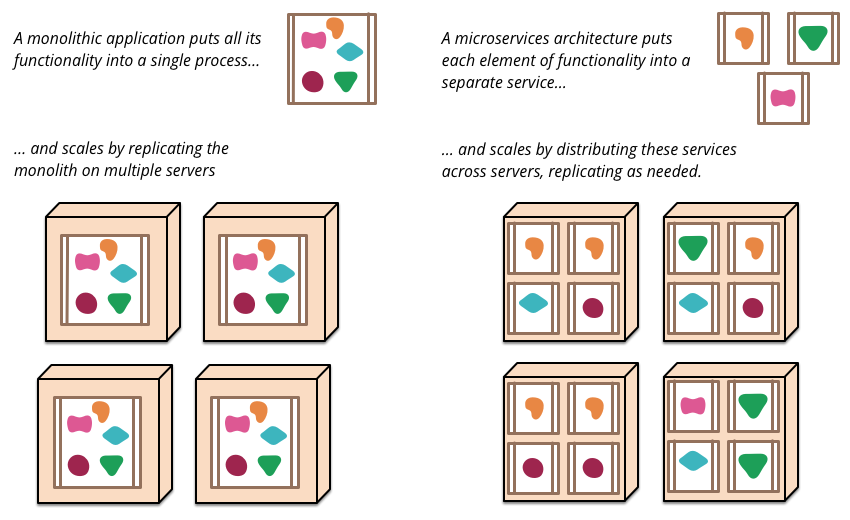
\includegraphics[scale=0.4]{microservices_escaling}
\caption{Los microservicios escalan de acuerdo a su carga de trabajo para asegurar la disponibilidad de la funcionalidad que ofrecen. \cite{Lewis2014}}
\end{figure}

\section{Los microservicios en la fase de requisitos}

La fase de requisitos del software es aquella en la que se elicitan, analizan, documentan, validan y mantienen los requisitos del sistema. Los requisitos del software expresan las necesidades y restricciones asociadas a un sistema. \cite{Fernandes2016} El artefacto principal que se produce en esta fase es el documento con la especificación de requisitos software (ERS). Una vez validado dicho documento por los stakeholders se puede iniciar la fase de diseño la solución. Esto no significa el final de esta fase del proceso: la gestión de los requisitos continúa durante el resto del desarrollo del producto.

\subsection{Requisitos funcionales y no funcionales}

Los requisitos se pueden clasificar en funcionales y no funcionales. Los \textbf{requisitos funcionales} (RF) describen la funcionalidad que los usuarios esperan del sistema. Los \textbf{requisitos no funcionales} (RNF) son restricciones impuestas sobre el sistema a desarrollar, estableciendo por ejemplo como de rápido o fiable ha de ser. Mientras que los primeros no incluyen ninguna mención relacionada con la tecnología que emplea el sistema, los segundos sí pueden establecer restricciones de este tipo. Por ejemplo, un requisito no funcional puede consistir en desarrollar una aplicación en un lenguaje de programación específico o hacer que esté disponible para diferentes sistemas operativos móviles. Por este motivo, los requisitos deben ser tenidos en cuenta a lo largo de todo el desarrollo del sistema.

Los requisitos funcionales y no funcionales son ortogonales en el sentido de que diferentes diseños de software pueden ofrecer la misma funcionalidad (RF) pero con distintos atributos de calidad (RNF). Los arquitectos software están más centrados en los requisitos no funcionales porque estos son los que conducen hacia la elección de una u otra arquitectura. Los requisitos no funcionales pueden influir en los patrones arquitectónicos a seguir, las futuras estrategias de implementación del sistema o la plataforma sobre la que se desplegará el sistema. \cite{Ameller2013}

\begin{figure}[h]
\centering
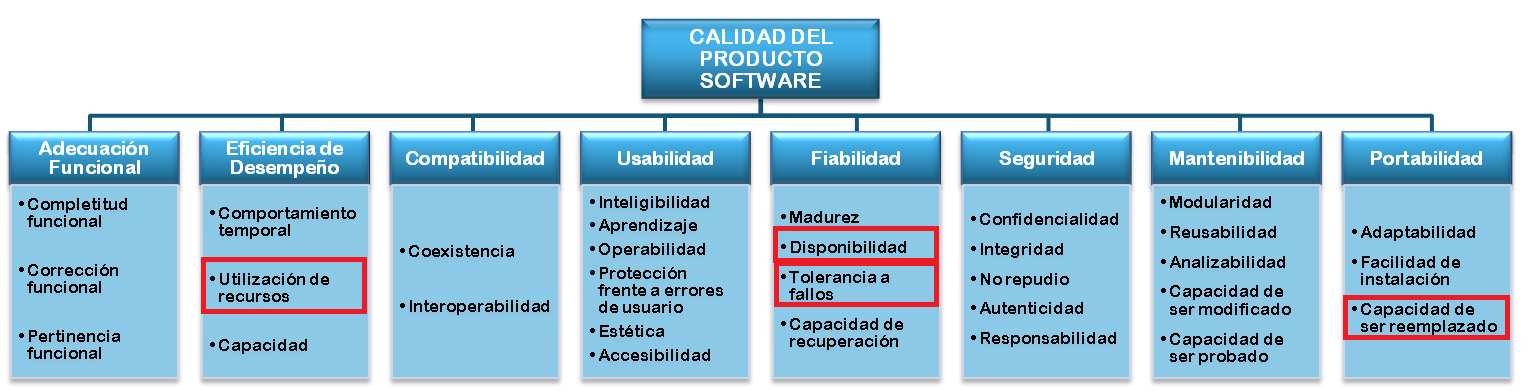
\includegraphics[scale=0.5]{iso25010}
\caption{Características y subcaracterísticas definidas en el modelo de calidad del producto de la ISO/IEC 25010. \cite{Standard2010}}
\end{figure}

Requisitos no funcionales asociados a atributos de calidad como la tolerancia a fallos o la disponibilidad pueden conducir al arquitecto hacia la elección de una arquitectura basada en microservicios:

\begin{itemize}

\item La \textbf{tolerancia a fallos} se define en la ISO/IEC 25010 como la capacidad del sistema para operar según lo previsto en presencia de fallos hardware o software. \cite{Standard2010} Cuando se escala un sistema, la probabilidad de fallo es inevitable. Muchas organizaciones invierten mucho esfuerzo en evitar que un fallo se produzca, pero muy poco en mecanismos para recuperar el sistema una vez se ha producido. Un sistema que por culpa de un servicio caído deja de funcionar es menos resilente que un sistema que puede continuar ofreciendo el resto de sus funcionalidades.

\item La \textbf{disponibilidad} se define como la capacidad del sistema de estar operativo y accesible para su uso cuando se requiere. \cite{Standard2010} En los sistemas distribuidos existen 3 características sobre las que se debe hacer balance: la consistencia, que establece que vamos a obtener una respuesta correcta de cualquier nodo de un servicio de acuerdo a su especificación, la disponibilidad, que ya hemos definido, y la tolerancia a particiones, que es la habilidad de gestionar situaciones en las que la comunicación entre las partes de un sistema se interrumpe. El teorema de CAP (debe sus siglas a las características en inglés Consistency, Availability y Partition Tolerance) establece que en caso de fallo, solo dos de las tres características pueden prevalecer. \cite{Gilbert2012}

\end{itemize}

\subsection{El teorema de CAP}

Pongamos un ejemplo en el que un microservicio está replicado y se produce un fallo por el cual la comunicación entre las replicas se interrumpe y los cambios en una replica no se pueden propagar al resto. Los \textbf{sistemas AP} son los sistemas que surgen fruto de sacrificar la consistencia cuando un fallo se produce, mientras que en los \textbf{sistemas CP} se pierde la disponibilidad. 

En el primer tipo, las replicas continuarían operativas, pero como los datos entre las replicas no se sincronizan se pueden obtener datos incorrectos al hacer una consulta. Cuando la comunicación se restablece, los cambios entre las replicas se sincronizarán. En los sistemas CP, para mantener la consistencia entre las replicas se tiene que rechazar cualquier petición, con lo que el servicio deja de estar disponible.

Los sistemas AP escalan más fácilmente y son más sencillos de construir, pero nos obligan a una consistencia eventual de los datos. Los segundos son los únicos que nos aseguran una consistencia fuerte, pero son más difíciles de construir. A la hora de optar por una solución u otra se debe tener en cuenta la especificación de requisitos, donde se debe detallar de forma específica y cuantitativa cuánto tiempo puede nuestro servicio estar inoperativo o con un dato obsoleto. Si en las fases siguientes se opta por una arquitectura basada en microservicios, no será necesario implementar el sistema completo de una u otra forma. Cada microservicio tendrá necesidades diferentes y podrá seguir la aproximación que mejor le convenga. \cite{Newman2015a}

\section{Los microservicios en la fase de diseño} \label{sct:FaseDiseño}

En la fase de diseño se definen la arquitectura, componentes e interfaces del sistema. La especificación de requisitos es analizada para producir una descripción de la estructura interna del sistema, con el suficiente nivel de detalle para que sirva como base en su construcción. En esta fase se plantean diferentes diseños como alternativas de las que se debe hacer balance. Los modelos que se generan se emplearán para validar que se cumplen los requisitos establecidos y para planificar la fase de implementación. \cite{Bourque2014}

\subsection{Librerías versus servicios} \label{subsect:librerias}

Un componente es una unidad de software que se puede reemplazar y actualizar de forma independiente. Las \textbf{librerías} son componentes que están ligados a un programa y son invocadas a través de llamadas a funciones. En cambio, los \textbf{servicios} son componentes que se ejecutan como procesos externos y con los que se puede comunicar a través de mecanismos como llamadas a procedimientos remotos (RPC) o peticiones HTTP. \cite{Lewis2014}

Uno de los motivos por los que se recomienda emplear servicios frente a librerías es que los servicios se pueden desplegar de forma independiente. Solo algunos cambios en la interfaz o contrato del servicio requerirán un cambio en sus consumidores. Además, algunas librerías obligan al uso específico de una tecnología. Sin embargo, las llamadas remotas son más costosas que las invocaciones dentro del mismo proceso, por lo que la interfaz del servicio debe definirse de tal forma que sus consumidores no tengan que comunicarse con él continuamente.

\subsection{Diseño guiado por el dominio (DDD)}

El \textbf{diseño guiado por el dominio} (DDD) es un enfoque para el desarrollo de software que propone un modelado rico, expresivo y evolutivo basado en la realidad del negocio. El dominio representa lo que hace una organización y la forma en qué lo hace.

Con esta aproximación los expertos del dominio y los desarrolladores se sitúan en el mismo nivel empleando un lenguaje ubicuo. No hace falta ninguna traducción de términos entre ellos porque todos hablan un lenguaje común, que se plasma hasta en el código de programación. El lenguaje no tiene porque seguir los estándares de la industria que representa: emplea los términos y acciones que en el negocio se dan. \cite{Vaughn2013}

El lenguaje ubicuo que se emplea crece y cambia con el paso del tiempo. Nadie es capaz de conocer el dominio de un negocio completo porque este forma parte de un proceso de descubrimiento continuo. Si la organización sigue una estrategia de desarrollo ágil, en cada iteración se refina el modelo de forma incremental y este plasma en todo momento el software en funcionamiento.

Para su tratamiento, las áreas independientes del dominio se transforman en contextos delimitados. Cada contexto delimitado es un límite explícito que tiene su propio lenguaje ubicuo. Un concepto tiene un significado dentro de un contexto delimitado, pero fuera de él puede tener un significado totalmente distinto. No se puede tratar de incluir todos los conceptos en un único contexto: se deben separar los conceptos en diferentes contextos y entender las diferencias que existen para un concepto llamado igual en uno y otro contexto.

\begin{figure}[h]
\centering
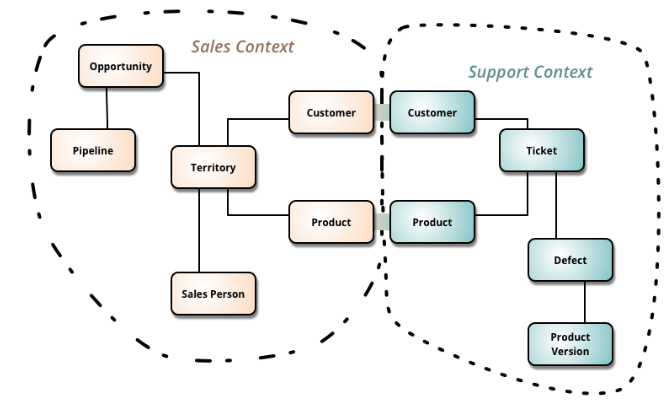
\includegraphics[scale=0.8]{bounded_contexts}
\caption{Ejemplo de dos contextos delimitados dentro del mismo dominio que emplean el mismo nombre para un concepto, pero con significados diferentes. \cite{Fowler}}
\label{fig:BoundedContexts}
\end{figure}

Cada contexto está formado por modelos que no necesitan ser compartidos con otros a menos que se defina explícitamente una interfaz que los empleen. La interfaz es el punto de entrada para que otros contextos puedan comunicar con el nuestro, empleando los términos y entidades que en nuestros modelos se definan.

Esta perspectiva puede trasladarse fácilmente al modelado de microservicios. Los contextos delimitados que analicemos en nuestro sistema son firmes candidatos a transformarse en servicios. Así, los límites de un servicio quedan bien limitados porque  todas las entidades que pueda requerir se encuentran dentro de sus fronteras, garantizándose su alta cohesión y bajo acoplamiento. \cite{Newman2015a}

\subsection{Descomposición en microservicios} \label{subsect:Descomposicion}

Cuando se razona sobre los límites de un servicio no se debe pensar en los datos que este almacena sino en las funcionalidades que ofrece. Pensar en los datos que almacena nos conduce a desarrollar únicamente servicios CRUD (en inglés, aquellos que nos permiten las operaciones de crear, leer, actualizar y eliminar datos), que ofrecen unas operaciones muy limitadas. Un servicio ofrece ciertas funcionalidades o capacidades que aportan \textbf{valor al negocio}.

Una descomposición temprana de un sistema en microservicios puede conllevar ciertos riesgos. Si el equipo a cargo del desarrollo tiene pocos conocimientos del dominio del problema a resolver, puede  ser buena idea comenzar la implementación como si de un sistema monolítico se tratara. Un mal diseño inicial puede desenvocar en que dos servicios se tengan que combinar porque exista un exceso de interacciones entre ellos. 

Es aconsejable dividir la solución en grandes servicios que poco a poco se vayan dividiendo en más pequeños conforme se estudien las ventajas de hacer cada nueva extracción. Una vez sean conocidos los límites de cada servicio, se pueden refactorizar el código y los datos hacia una granularidad más fina. Como se puede ver en la figura, se puede migrar primero solo la funcionalidad del servicio sin preocuparse por sus límites en base de datos para no tener que realizar simultáneamente dos migraciones. Una vez nos aseguremos de que el servicio funciona correctamente, podemos migrar sus datos a una base de datos diferentes ya que cada servicio ha de ser dueño de sus propios datos. \cite{Richards2016}

\begin{figure}[h]
\centering
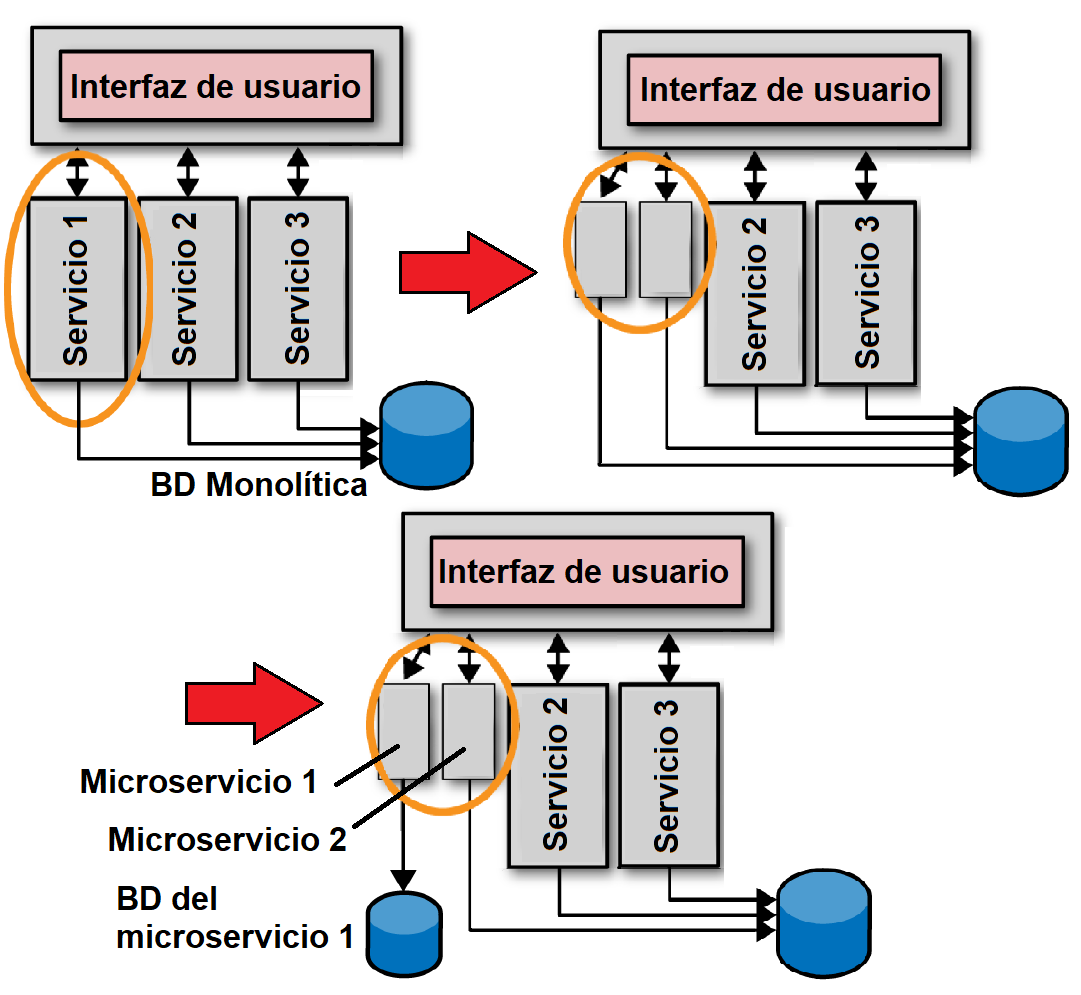
\includegraphics[scale=0.4]{refactoring}
\caption{Primero, se dividen los grandes servicios en microservicios. Una vez hecho esto, se migran sus datos. \cite{Richards2016}}
\end{figure}

Cuando sea necesario realizar un cambio por nuevos requisitos del negocio, estos se localizarán en un contexto bien delimitado porque existirá una correspondencia entre la estructura de la organización y los microservicios del sistema. Como consecuencia, el tiempo medio para realizar un cambio se verá reducido porque solo hará falta volver a desplegar una porción del sistema. Además, la comunicación entre microservicios se asemejará a la existente entre las entidades del negocio.

\subsection{La tarea del arquitecto de software}

El software ha de ser diseñado para ser flexible, adaptarse y evolucionar en función de los requisitos de los usuarios. En lugar de centrarse en diseñar un producto final perfecto, el arquitecto debe crear un entorno donde el sistema correcto pueda emerger creciendo progresivamente a medida que se descubren nuevos requisitos. Gracias a su modularidad, los microservicios son el entorno perfecto para que esto ocurra.

El arquitecto de software debe preocuparse más por como interaccionan los servicios entre ellos y no tanto en lo que ocurre dentro de sus límites. En organizaciones grandes, cada microservicio puede estar desarrollado por un equipo distinto y es el arquitecto quien debe hacer de puente entre ellos. \cite{Newman2015a}

Una de las ventajas de las arquitecturas basadas en microservicios es la \textbf{heterogeneidad tecnológica}: cada servicio puede ser desarrollado empleando una pila tecnológica distinta. No obstante, dejar plena libertad a cada equipo para elegir la tecnología del servicio que va a desarrollar puede traer problemas a la hora de integrarlo con el resto del sistema. El uso de contratos o establecer normas en aspectos clave como el protocolo de comunicación entre los servicios facilitará su consumo. Las decisiones de diseño de un servicio en particular pueden recaer en el equipo responsable. En este caso, el arquitecto solo juega un papel de supervisor y asesor para evitar que se pierda la imagen del sistema completo.

\section{Los microservicios en la fase de implementación}

La fase de implementación consiste en la creación de un sistema o componente software combinando técnicas de programación, verificación y depuración. Esta fase emplea la salida de la fase de diseño y sirve como entrada para la de pruebas. Los límites entre estas tres fases varían en función del proceso seguido. \cite{Bourque2014}

\subsection{Integración de microservicios}

La \textbf{integración} es la parte más relevante en los sistemas basados en microservicios. Hacerlo correctamente nos asegurará su autonomía y su despliegue de manera independiente.

Por un lado, la tecnología empleada para la comunicación entre servicios no debe restringir la tecnología empleada en estos. Por otro lado, los consumidores deberían de tener total libertad en la tecnología que emplean y consumir un servicio para ellos no debe ser complejo de implementar. Además, los consumidores no deben conocer detalles internos del servicio que consumen para garantizar que estén desacoplados. \cite{Newman2015a} Existen muchas técnicas para la integración entre las que destacan: 

\begin{itemize}

\item \textbf{RPC} (Remote Procedure Call):la llamada a procedimiento remoto es una técnica que permite ejecutar una llamada a un servicio como si de una llamada local se tratara. No es necesario que cliente y servidor empleen la misma pila tecnológica, aunque algunas tecnologías como Java RMI (Remote Method Invocation) sí lo requieren. 

El formato de los mensajes también varía de una tecnología a otra. SOAP (proviene del inglés Simple Object Access Protocol) emplea XML (también del inglés eXtensible Markup Language) mientras que por ejemplo Java RMI transmite mensajes binarios.

\item \textbf{REST} (Representational State Transfer): la transferencia de estado representacional es un estilo arquitectónico inspirado en la Web. Se basa en el concepto de recurso, un objeto que el servicio conoce y del que puede crear diferentes representaciones bajo demando. La representación del recurso está completamente desacoplada de como se almacena.

La arquitectura REST es ampliamente usada junto con HTTP (término que proviene del inglés Hypertext Transfer Protocol). Los verbos que se definen en HTTP actúan sobre recursos: por ejemplo, con el verbo GET se puede obtener una representación del recurso y con el POST crear uno nuevo.

\item \textbf{Integración basada en eventos}: en la integración basada en eventos, un servicio publica un evento cuando sucede algo relevante. Al evento se suscriben aquellos componentes que deben reaccionar al evento producido. Para hacer llegar los eventos a sus consumidores se debe mantener una nueva infraestructura, como puede ser una cola basada en mensajes.

\begin{figure}[h]
\centering
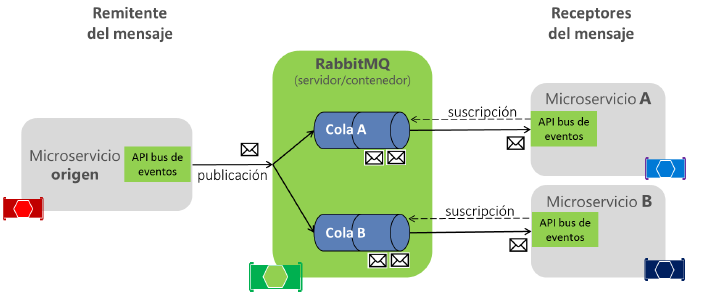
\includegraphics[scale=0.85]{rabbitmq}
\caption{Ejemplo de integración basada en eventos con un contenedor de RabbitMQ. \cite{DelaTorre2018}}
\end{figure}

Un bróker de mensajería es un patrón arquitectónico para la validación, la transformación y el enrutamiento de mensajes. RabbitMQ es un ejemplo de este patrón. En esta herramienta, el productor de un evento publica este a través de una API, donde será tramitado por el bróker para hacerlo llegar a todos los consumidores suscritos.
 
\end{itemize}

Tanto SOAP como REST emplean HTTP, aunque solo el segundo emplea los verbos definidos en HTTP. Existen pocas librerías para trabajar con SOAP, mientras que prácticamente cualquier lenguaje de programación contemporáneo cuenta con un cliente HTTP, con soporte para más o menos verbos. En cuanto a su rendimiento, REST es más eficiente en términos de latencia y ancho de banda consumido. \cite{Mulligan} REST es más recomendable que SOAP para enviar grandes volúmenes de datos por ser más compacto y permitir formatos como el JSON o el binario. Sin embargo, ni uno ni otro son recomendables para trabajar en redes con latencias bajas porque emplean HTTP. En este caso, es mejor emplear directamente protocolos como TCP o UDP. 

En cuanto al tercer tipo de integración, la integración basada en eventos fomenta la escalabilidad y resilencia de los servicios y reduce el acoplamiento entre ellos. No obstante, requiere aprovisionar nuevas infraestructuras y añade complejidad a la hora de razonar sobre el sistema por ser una comunicación asíncrona. Algunas buenas prácticas para afrontar su complejidad van desde el uso efectivo de sistemas de monitorización hasta el uso de identificadores de correlación para trazar las llamadas entre servicios. \cite{Newman2015a}

\subsection{Programación y persistencia políglotas} \label{subsec:Poliglota}

%TODO Sustituir anteriormente por enlace.
Como hemos comentado anteriormente, diferentes microservicios se pueden desarrollar empleando diferentes tecnologías. La base de datos que contiene los datos del servicio o la arquitectura interna del microservicio también pueden adaptarse a los requisitos del mismo. \cite{DelaTorre2018} La \textbf{programación políglota} se fundamenta en que diferentes lenguajes de programación son más aptos para tratar problemas específicos. Es más productivo escoger el lenguaje adecuado para un servicio concreto que tratar de buscar un lenguaje que se ajuste a los requisitos de todos.

\begin{figure}[h]
\centering
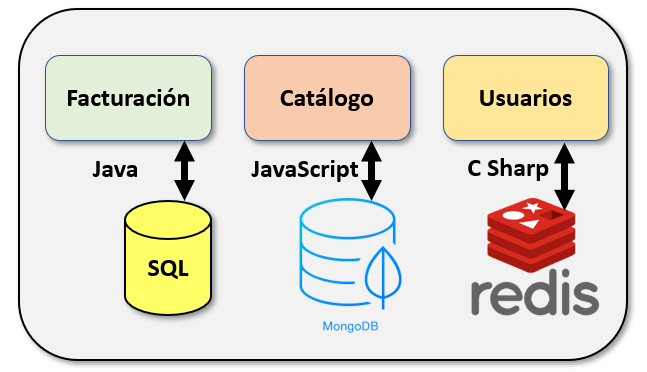
\includegraphics[scale=0.65]{poliglota}
\caption{Ejemplo de sistema políglota.}
\end{figure}

El término también se puede extrapolar a la persistencia. La \textbf{persistencia políglota} emplea diferentes tecnologías para la persistencia en función de los datos a almacenar y de cómo estos se van a manipular. Cada microservicio es dueño de sus datos y puede emplear una tecnología diferente. Las bases de datos relacionales no son la única opción y se deben considerar otras que escalen mejor si el servicio recibe muchas peticiones o se quiere hacer una explotación eficiente de los datos. \cite{Fowler2011}

En ambos casos, se debe hacer balance entre los beneficios que puede aportar un diseño políglota y sus costes asociados, por ejemplo, de aprendizaje.

\subsection{La ley de Conway}

Problemas asociados a bases de código inmensas donde colabora un gran equipo pueden ser evitados empleando microservicios. Si el código está repartido entre diferentes componentes, equipos pequeños pueden encargarse de mantener cada uno de ellos. De esta manera, la organización del trabajo adquiere un enfoque más ágil al estar formado por equipos independientes y auto-organizados.

%TODO Continuar ...

\section{Los microservicios en la fase de pruebas}
% Art of unit testing
% Building microservices
% Simian army

Las pruebas de software consisten en la verificación dinámica de que un programa produce las salidas esperadas para un conjunto finito de casos de prueba. Las pruebas son dinámicas porque se verifica el programa en ejecución. Los casos de prueba son finitos porque el número posible de pruebas es infinito y estos se seleccionan en función de la prioridad y riesgo del código bajo pruebas. Además, se debe comprobar la salida obtenida con el resultado esperado para comprobar si esta es o no aceptable. \cite{Bourque2014}

\subsection{Pruebas unitarias}

Una \textbf{prueba unitaria} es una pieza de código que invoca al método o clase bajo prueba y que comprueba ciertas asunciones sobre su lógica. Se ejecuta de forma rápida y sencilla, está automatizado y es fácilmente mantenible. \cite{Osherove2014} En general, se prefiere tener un gran número de este tipo de pruebas por su rapidez, porque pueden ayudar a la refactorización del código y porque es donde mayor cantidad de defectos se suele capturar.

\begin{figure}[h]
\centering
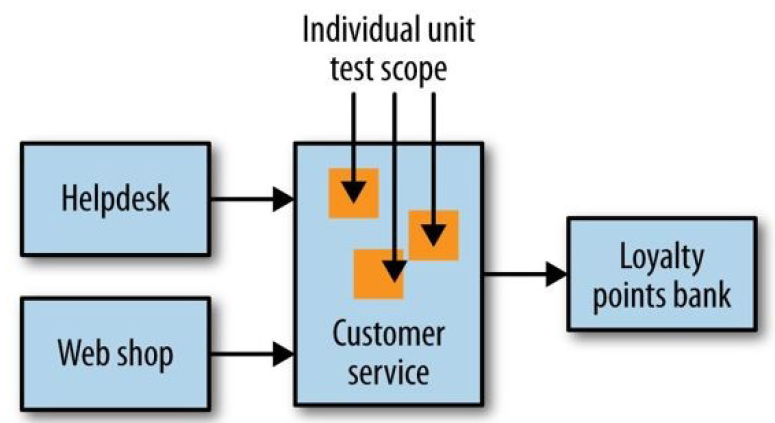
\includegraphics[scale=0.5]{Unit_Tests}
\caption{Diagrama de pruebas unitarias.}
\end{figure}

\subsection{Pruebas de servicios}

En las \textbf{pruebas de servicios} se verifica cada una de las funcionalidades que un servicio expone. Se pretende verificar el servicio de forma aislada y para ignorar las dependencias que el servicio bajo pruebas tiene sobre otros se reemplazan los servicios colaboradores por fakes.

Encajan dentro de las pruebas de integración, que se definen como la prueba como un conjunto de dos o más módulos de software que colaboran para evaluar un resultado esperado. \cite{Osherove2014} Este tipo de pruebas pueden ser igual de rápidas que las unitarias siempre que no se tengan que emplear un gran número de infraestructuras como bases de datos o colas.

\begin{figure}[h]
\centering
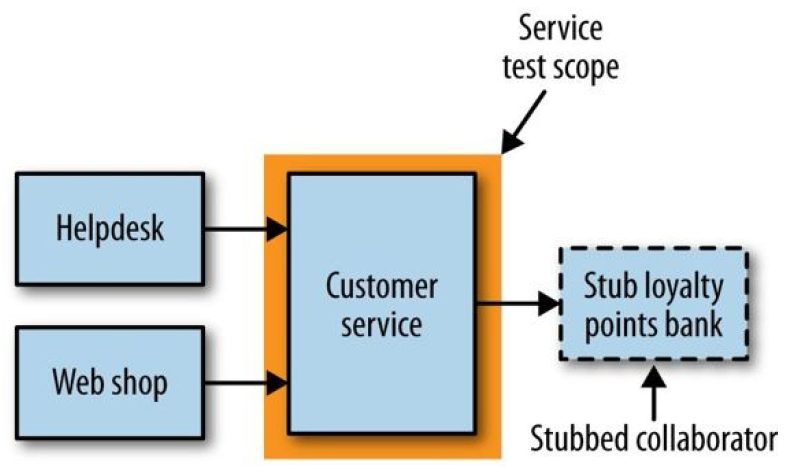
\includegraphics[scale=0.5]{Service_Tests}
\caption{Diagrama de pruebas de servicios.}
\end{figure}

\subsection{Pruebas de extremo a extremo}

Las \textbf{pruebas de extremo} a extremo son pruebas que se ejecutan sobre todo el sistema. Cubren gran parte de código, por lo que su correcta ejecución dan mucho grado de confianza. En su ejecución se levantan varios servicios diferentes.

Son pruebas frágiles: conforme el alcance de la prueba aumenta más son las partes sobre las que no se puede tener control. Estas partes pueden introducir fallos que no demuestran que la funcionalidad tenga un defecto y hacen la prueba menos determinista. Si la prueba falla continuamente, el equipo encargado puede llegar a asumir como normal está situación. Su tiempo de ejecución es mayor y en consecuencia, más tarde se detecta si un cambio ha introducido un defecto. \cite{Newman2015a}

\begin{figure}[h]
\centering
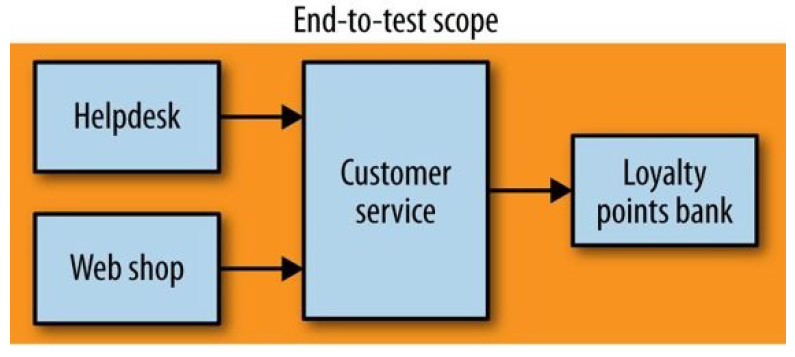
\includegraphics[scale=0.5]{End_To_End_Test}
\caption{Diagrama de pruebas de extremo a extremo.}
\end{figure}

\subsection{Balance de pruebas a realizar}

A medida que aumenta el alcance de las pruebas lo hace el nivel de confianza que las pruebas dan sobre la ausencia de defectos. Por otro lado, cuanto más arriba en la pirámide más tiempo tardará una prueba en implementarse y ejecutarse. Además, determinar el motivo de fallo de una prueba será más costoso cuanto mayor sean las líneas de código probadas. \cite{Cohn2010}

\begin{figure}[h]
\centering
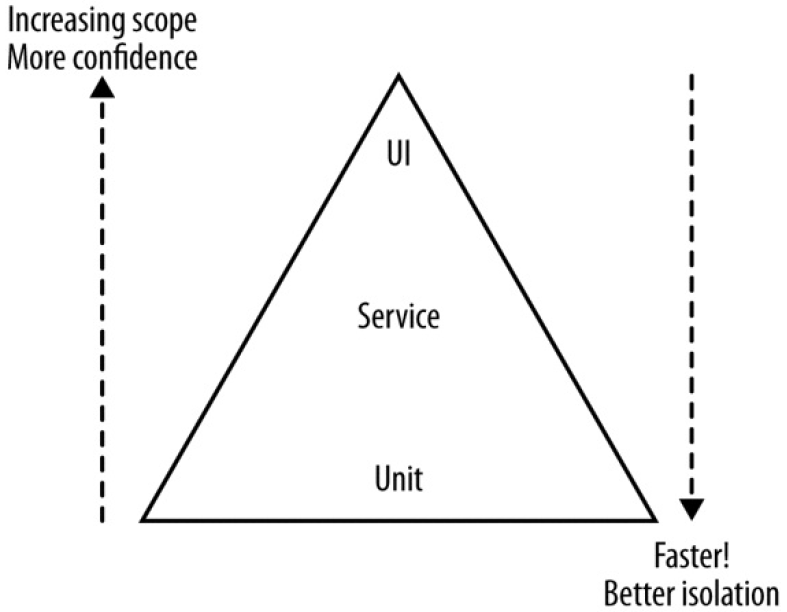
\includegraphics[scale=0.5]{Cohn_Pyramid}
\caption{Pirámide de pruebas diseñada por Mike Cohn. \cite{Cohn2010}}
\end{figure}

El número de pruebas que se aconseja tener de cada tipo aumenta conforme descendemos por la pirámide. El número de servicios que participan para ofrecer una funcionalidad al usuario puede ser muy alto y en una prueba no se deberían de levantar más de 3 o 4 servicios para no potenciar las desventajas que hemos mencionado. Por este motivo, las pruebas de extremo a extremo deben ser las mínimas posibles y se deben refactorizar en pruebas de servicios que empleen fakes siempre que se pueda.

\section{Los microservicios en la fase de despliegue}
% Docker
% Kubernetes
% Orquestadores (¿Moltó?)
% Azure y AWS
% CI/CD

El despliegue se define como la entrega de software (como un producto completo o como resultado de un incremento en un desarrollo incremental) al cliente para que este lo evalúe y devuelva retroalimentación al equipo de desarrollo. \cite{Pressman} Debido a la naturaleza incremental de la mayoría de procesos de desarrollo, esta es una actividad que se realiza numerosas ocasiones. 

En cada despliegue, se debe proveer del soporte necesario para el empleo de las nuevas características. Además, la retroalimentación recibida guiará el proceso de desarrollo hacia las siguientes modificaciones y funcionalidades que se deben realizar.

Los problemas que aparecen en una nueva versión del producto deben ser atendidos. Para garantizar que estos no ocurran, se deben hacer pruebas en cuantos más entornos posibles mejor.

\subsection{Integración y entrega continua}

La \textbf{integración continua} es una práctica en el desarrollo de software donde los miembros del equipo integran su trabajo de forma frecuente, normalmente a diario. Cada integración se verifica mediante compilaciones automatizadas que incluyen la ejecución de pruebas para detectar errores y conflictos en la integración. \cite{Fowler2006} El término tiene su origen como una de las doce prácticas de la metodología Extreme Programming (XP).

Durante este proceso se crean artefactos sobre los que se ejecutarán validaciones. Los artefactos construidos deben ser lo más parecidos a los que más tarde se despliegan en la versión de producción para asegurar que es el mismo artefacto sobre el que se han hecho las pruebas. Entre los beneficios de la integración continua encontramos:
 
\begin{itemize}

\item \textbf{Rápida retroalimentación}: los desarrolladores obtienen más rápido una respuesta sobre la calidad de sus cambios. Con este fin, la compilación ha de ser lo más rápido posible. Se pueden obtener mayores beneficios de la integración continua a través de las compilaciones por fases o build pipelines. En este tipo de compilaciones se separa por pasos el proceso. Los pasos de la pipeline pueden ser manuales, como las pruebas de aceptación de un usuario, o estar automatizados, como la ejecución de pruebas unitarias. La ventaja de hacer esto es que se obtiene una retroalimentación más rápida si se ejecutan de forma separada acciones rápidas de otras más pesadas. \cite{Fowler2006}

\item \textbf{Equipo sincronizado}: los integrantes de un equipo obtienen más rápido los cambios que otros han realizado y conocen en todo momento el estado de la compilación. Si esta falla, arreglarla es la prioridad número uno.

\item \textbf{Trazabilidad}: si el código está bajo control de versiones, en cualquier momento se puede volver a construir un artefacto de una versión concreta a partir del código que la origina. \cite{Newman2015a}

\end{itemize}

\begin{figure}[h]
\centering
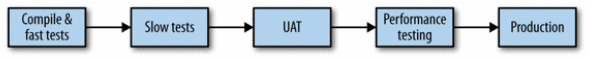
\includegraphics[scale=1]{pipeline}
\caption{Ejemplo de una pipeline. \cite{Newman2015a}}
\end{figure}

La \textbf{entrega continua} extiende la idea de la integración continua en cuanto a que cada cambio que ha superado la compilación puede ser candidata para ser desplegada en producción en cualquier momento. Sobre cada cambio se puede decidir si se publica o no a producción y hacerlo no cuesta más que pulsar un botón porque está todo el proceso de despliegue automatizado. La práctica de que cada cambio que se realiza y supera la pipeline es publicado automáticamente a producción se denomina \textbf{despliegue continuo}. \cite{Fowler2013}

\subsection{Virtualización y tecnología de contenedores}

Un \textbf{host} representa una unidad genérica de aislamiento, un sistema operativo donde se pueden instalar y ejecutar servicios. Si desplegamos directamente sobre máquinas físicas, entonces un host será el equivalente a una de ellas. Sin embargo, tener muchos hosts es costoso si cada uno consiste en una máquina diferente. \cite{Newman2015a}

La \textbf{virtualización} nos permite dividir una máquina en hosts separados, donde pueden ejecutarse servicios distintos. En la virtualización tradicional, cada una de las máquinas virtuales (MV) puede ejecutar su propio sistema operativo. Un recurso adicional es añadido entre la máquina física y las virtuales: el hipervisor. El hipervisor reparte recursos de la máquina física como la CPU o la RAM entre los distintos hosts virtualizados y permite al usuario la gestión de las máquinas virtuales contenidas.

El mayor inconveniente de las máquinas virtuales es que se puede dividir una máquina en muchas piezas como queramos porque la separación entre los hosts supone un coste. El hipervisor también consume recursos y cuantas más son las máquinas que debe gestionar, mayor será su consumo. Además, el tiempo de puesta en funcionamiento de una máquina virtual es de la magnitud de minutos, mientras que el arranque de un contenedor ronda los pocos segundos. \cite{Dua2014} Esto es muy importante en desarrollos que siguen las técnicas de integración continua donde se despliegan artefactos frecuentamente. 

Los \textbf{contenedores} son sistemas operativos ligeros que se ejecutan sobre una máquina con la que comparten el kernel. El número de contenedores que una máquina puede alojar es mayor que el número de máquinas virtuales debido a la naturaleza ligera de estos. \cite{Dua2014} Su uso de recursos es y tiempo de aprovisionamiento son menores al de una MV, lo que reduce el tiempo de retroalimentación sobre el funcionamiento de un servicio. Sin embargo, el grado de aislamiento de los contenedores no es perfecto ya que existen formas en las que se puede interferir en el funcionamiento de otro contenedor debido a problemas de diseño y bugs conocidos. \cite{Newman2015a}

\begin{figure}[h]
\centering
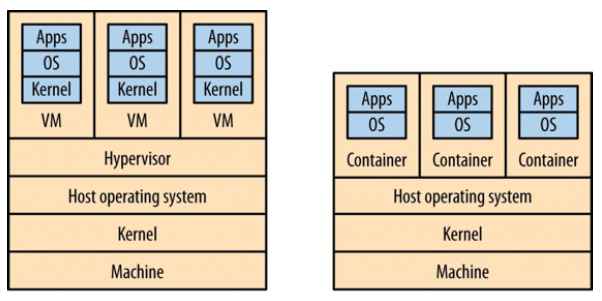
\includegraphics[scale=0.8]{containers_vms}
\caption{Comparación entre la virtualización y la contenerización. \cite{Newman2015a}}
\end{figure}

Ambas soluciones se pueden combinar para obtener las ventajas de ambas. Se puede obtener una máquina virtual de una plataforma como Amazon Web Services (AWS) que nos asegure características como la escalabilidad bajo demanda y sobre ella ejecutar diferentes servicios desplegados como contenedores.

\section{Los microservicios en la fase de mantenimiento}
% You code, you run it -> Buscar documento "oficial"
% Monitorización
% Arquitectura evolutiva

Los productos software cambian y evolucionan. Una vez están desplegados en el entorno donde operan se dan situaciones en las que se detectan errores o los requisitos de los usuarios se ven modificados. Es una fase que debe comenzar de forma temprana para garantizar la mantenibilidad del sistema a desarrollar. \cite{Bourque2014}

El mantenimiento de software es la fase del desarrollo que más recursos consume, alrededor del 60\% o 70\% del coste de un proyecto. La mayoría del software que hoy se emplea tiene entre 10 y 15 años, tiempo en el cual ha sufrido muchas modificaciones hasta alcanzar un diseño pobre y difícil de mantener. Se puede definir el software mantenible como aquel que se diseña de forma modular, siguiendo patrones de diseño y estándares de calidad y que se documenta de tal forma que es explicativo por si mismo. \cite{Pressman} 

Gracias a su diseño modular, los microservicios son una arquitectura que se puede seguir para hacer más sencillo el mantenimiento de un sistema. Sin embargo, las consecuencias de elegir un estilo arquitectónico no son evidente hasta años más tarde de haber sido tomadas, por lo que hasta que no se vean sistemas maduros que empleen microservicios no se debe afirmar a ciencia cierta que garantizan estas características. \cite{Lewis2014}

\subsection{Reemplazamiento}

En la mayoría de empresas abundan los sistemas legados que nadie desea mantener. La \textbf{refactorización} de estos sistemas es imposible por su tamaño y riesgo. Si en lugar de haber empleado una arquitectura monolítica para su diseño se emplearan microservicios se observaría como los barreras para la refactorización no existen al poderse reescribir el microservicio al completo en pocos días.

Una regla que puede ser aplicada es establecer un tamaño para un microservicio tal que pueda ser completamente reescrito en 2 semanas. \cite{Newman2015a}

\subsection{You Build It, You Run It}

En muchas organizaciones, el desarrollo de sistemas se hace a través de proyectos: piezas de software que una vez desarrolladas se consideran completadas. En una aproximación basada en microservicios, cada equipo es responsable del ciclo de vida completo de un producto o servicio. Esto sigue la filosofía de Amazon: \textbf{"you build, you run it"}. \cite{Lewis2014}

No hay necesidad de distinguir entre quien construye un sistema y quien lo ejecuta y posteriormente mantiene. Esta filosofía aproxima a desarralloradores y clientes: los desarrolladores están en contacto directo con los clientes día tras día, lo que les proporciona retroalimentación para mejorar la calidad de sus servicios. Tampoco hay necesidad de contar en la organización con un equipo centrado en la infraestructura (IT). Contar con un equipo así distribuye la responsabilidad de hacer un servicio funcionar entre diferentes equipos y añade un sobreesfuerzo de coordinación y comunicación cuando un problema aparece. \cite{Vliet2011}

\subsection{Documentación}

Una de las ventajas de los microservicios es que acelara el proceso de desarrollo. Sin embargo, cuanto más rápido tratamos de implementar un servicio más probable es que tomemos atajos para poder desplegar antes una iteración del producto, lo que se traduce en un aumento de la \textbf{deuda técnica}. \cite{FowlerSusan}

En un equipo de desarrollo el conocimiento de cómo funciona un sistema se reparte entre los miembros que lo forman. Nadie es capaz de conocer completamente su funcionamiento y lo más probable es que cada desarrollador conozca mejor la parte donde más tiempo ha invertido. A la hora de realizar un cambio, el entendimiento de cómo funciona el sistema tiene que ser compartido por todos sus miembros para asegurar que el cambio a implementar es el correcto.

La documentación es una de las mejores maneras de solventar la deuda técnica y garantizar que el equipo de desarrollo conoce realmente cómo funciona un microservicio. Cabe recordar que cada microservicio puede seguir una arquitectura diferente o emplear una tecnología distinta. Debido a esto, se debe documentar de forma exhaustiva para facilitar la integración entre ellos y facilitar el traslado de personas de un equipo a otro.

\subsection{Monitorización}

Durante el mantenimiento se debe asegurar la disponibilidad de los microservicios. Las herramientas de monitorización son clave para garantizar los \textbf{acuerdos de nivel de un servicio} (SLA) y el estudio de errores cuando estos ocurren.

Con este propósito, se debe registrar toda aquella información relevante que ocurra. Los microservicios colaboran entre ellos para ofrecer funcionalidades concretas y recrear un sistema donde ha ocurrido un error puede ser complejo debido a que cada uno se versiona de forma independiente. Por ello, lo mejor es contar con toda la información necesaria registrada para determinar la causa del problema.

La información más útil se debe mostrar de forma gráfica a través de dashboards que reflejen el estado de salud de los servicios. Así, la informacón más consultada se puede visualizar de forma rápida y fácil de entender para ahorrar tiempo. No obstante, cuando un problema ocurre se debe hacer uso de alertas para atenderlo de forma prioritaria. Estas alertas han de ser accionadas automáticamente por métricas que superen un límite establecido, como puede ser el uso de recursos, o por la ocurrencia de excepeciones en el servicio. \cite{FowlerSusan}

%%%%%%%%%%%%%%%%%%%%%%%%%%%%%%%%%%%%%%%%%%%%%%%%%%%%%%%%%%%%%%%%%%%%%%%%%%%%%%%
%              					Estado del arte
%
%%%%%%%%%%%%%%%%%%%%%%%%%%%%%%%%%%%%%%%%%%%%%%%%%%%%%%%%%%%%%%%%%%%%%%%%%%%%%%%

\chapter{Estado del arte de la tecnología de microservicios}

\section{Contenedores}

\subsection{Docker}

Docker es una herramienta basada en contenedores Linux para la creación de artefactos que se pueden desplegar en cualquier entorno y se pueden distribuir y escalar bajo demanda. \cite{Matthias} Su funcionamiento es sencillo: en un fichero llamado \textbf{Dockerfile} se especifican las dependencias del servicio en distintos pasos y un comando que inicia el servicio. De la compilación del Dockerfile se origina una \textbf{imagen}, un paquete con todas las dependencias e información necesaria para crear un contenedor. Las imágenes permiten empaquetar un servicio para desplegarlo de forma confiable y reproducible tantas veces como se desee. \cite{DelaTorre2018}

La filosofía de Docker se centra en los contenedores desechables. Nada en el entorno donde se ejecuta la aplicación permanecerá ahí más allá de lo que viva la aplicación, por lo que no se delegará en entornos donde se encuentra casualmente una dependencia no especificada en la imagen. Docker promueve las arquitecturas sin estado (stateless) o que externalizan este a otras infraestructuras como bases de datos. Las aplicaciones así se hacen más portables, escalables y confiables. \cite{Matthias}

El proceso de desarrollo también se simplifica: en aproximaciones como la de microservicios, un equipo encargado de un servicio solo necesita la imagen de otro para integrarlo con el suyo y no necesita conocer detalles internos de este. Además, las tareas de construcción de la imagen, provisión de la configuración y despliegue pueden ser realizadas por diferentes personas, como se muestra en la figura. 

\begin{figure}[h]
\centering
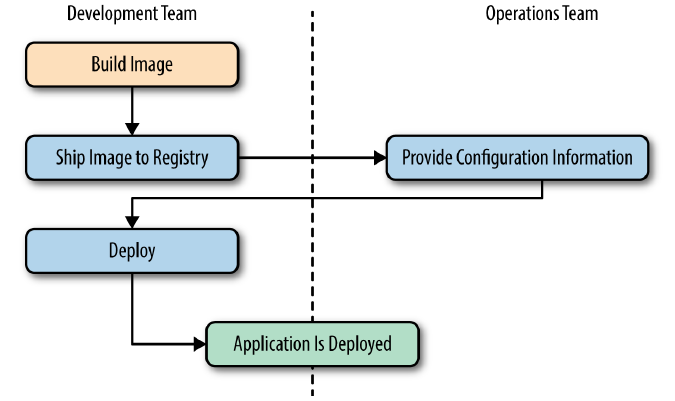
\includegraphics[scale=0.7]{docker_process}
\caption{Proceso de despliegue con Docker. \cite{Matthias}}
\end{figure}


Si se integra dentro del proceso de despliegue, cada cambio que pasa por una pipeline puede construir una nueva imagen Docker sobre la que se ejecutan pruebas de forma automatizada para después ser publicada a producción. De esta forma el equipo puede asegurarse de que el artefacto sobre el que se han ejecutado las pruebas es el mismo que se publica más tarde. 

\subsection{Vagrant}

\section{Orquestadores}

\subsection{Kubernetes}

Kubernetes es una herramienta diseñada por Google para el despliegue y orquestación de aplicaciones en contenedores Docker de forma resilente. Cada una de las máquinas que aloja uno o más contenedores Docker se denomina \textbf{nodo}. La unidad más pequeña con la que trabaja Kubernetes no son los contenedores, sino los pods. Un \textbf{pod} es una colección de contendores y volúmenes agrupados juntos en un nodo. Los \textbf{volúmenes} son sistemas de archivos virtuales que se pueden emplear para comunicar entre ellos a los contenedores de un nodo. Kubernetes orquesta a nivel de los pods, por lo que dos contenedores en el mismo pod serán administrados igual. \cite{Rensin2015}

\begin{figure}[h]
\centering
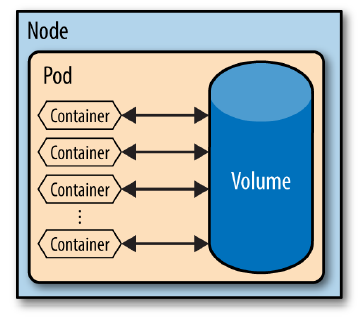
\includegraphics[scale=0.7]{kubernetes}
\caption{Un nodo de Kubernetes. \cite{Rensin2015}}
\end{figure}

Kubernetes se emplea principalmente para especificar el número de replicas que se desea tener simultánemanete de un pod. La herramienta es buena para asegurar la disponiblidad de un servicio, pero no garantizan la escalabilidad de este, que consistiría en modificar el número de replicas de un pod de forma dinámica en función de su demanda. Para este propósito se deben introducir balanceadores de carga como puntos de entrada al sistema. Estos balancenadores redirigirían cada petición al pod correspondiente y se encarguen de ajustar el número de replicas de un pod según una serie de reglas.

\subsection{Docker Swarm}


\section{Infraestructura}

\subsection{Microsoft Azure}

\subsection{Amazon Web Services (AWS)}

\section{Crítica al estado del arte}
% Trabajos presentados en la ETSINF.

\section{Propuesta}
%TODO Revisar

El lenguaje de programación que se va a emplear es C\# junto con el entorno de desarrollo (IDE) Visual Studio Enterprise 2017. Entre las plataformas de destino que ofrece la tecnología .NET vamos a utilizar tanto .NET Standard 2.0 como .NET Core en su versión 2.1, publicada en Mayo de 2018. \footnote{ Versiones de .NET Core 2.1: https://www.microsoft.com/net/download/dotnet-core/2.1} El uso de librerías distintas a las provistas por la plataforma se realizará a través de paquetes NuGet, un mecanismo sencillo que envuelve el código compilado de una librería y referencia a las dependencias de esta. \footnote{ Una introducción a NuGet: https://docs.microsoft.com/es-es/nuget/what-is-nuget}

Para el desarrollo de la interfaz de usuario se va a utilizar Xamarin.Forms. Xamarin es una plataforma que permite desarrollar aplicaciones móviles para dispositivos Universal Windows Platform (UWP), Android y iOS empleando código C\#. Xamarin.Forms es un conjunto de herramientas para Xamarin centrado en el desarrollo multiplataforma. Su propósito que se pueda compartir la mayor cantidad de código posible en el desarrollo de una aplicación para las distintas plataformas que hemos mencionado. \footnote{ Introducción a Xamarin.Forms
: https://docs.microsoft.com/es-es/xamarin/xamarin-forms/get-started/introduction-to-xamarin-forms}

A nivel de infraestructura se ha empleado Microsoft Azure para la persistencia de datos en la nube y para la exposición de servicios a través de Azure App Service y Azure Kubernetes Service (AKS). Microsoft Azure es una plataforma que ofrece un conjunto de herramientas y servicios en la nube. Tanto App Service como AKS son parte de sus servicios. El primero se emplea para crear aplicaciones en la nube de forma rápida sin necesidad de administrar la infraestructura sobre la que se hospeda. En cuanto al segundo, permite la orquestación de contenedores Docker a través de Kubernetes dentro de la infraestructura de Azure. \footnote{ Página oficial de Microsoft Azure: https://azure.microsoft.com/es-es/}

Para terminar, para las pruebas a nivel de API se ha empleado Postman. Postman es un entorno para el desarrollo de APIs (ADE) que nos va a permitir crear y almacenar de forma sencilla llamadas HTTP hacia la API del back-end. \footnote{ Página oficial de Postman: https://www.getpostman.com/}

%%%%%%%%%%%%%%%%%%%%%%%%%%%%%%%%%%%%%%%%%%%%%%%%%%%%%%%%%%%%%%%%%%%%%%%%%%%%%%%
%                       Especificación de requisitos                                 %
%%%%%%%%%%%%%%%%%%%%%%%%%%%%%%%%%%%%%%%%%%%%%%%%%%%%%%%%%%%%%%%%%%%%%%%%%%%%%%%

\chapter{Especificación de requisitos del caso de estudio}

\section{Descripción del caso de estudio}

Se desea desarrollar un sistema para la venta de productos electrónicos a través de dispositivos móviles. La aplicación móvil estará destinada solo a los clientes de una tienda, que deberán registrarse para usarla.

Los clientes podrán consultar los \textbf{productos} disponibles en la tienda junto con su precio, descripción y número de unidades en stock. Un \textbf{pedido} se define como un conjunto de productos que el cliente ha seleccionado junto con el número de unidades de cada uno. Mientras no se haya confirmado el pedido, se podrán añadir y eliminar productos al pedido en elaboración.

Todos los pedidos realizados por un cliente se mostrarán en un listado junto con el estado de los mismos. Para cada pedido, el cliente podrá generar una \textbf{factura} donde se listen los productos que lo componen y el precio total.

Una vez un cliente haya confirmado un pedido, este deberá ser aprobado por un empleado para ser entregado. Cuando esto suceda, se enviará una \textbf{notificación} al correo electrónico del cliente. Mientras que el empleado no lo apruebe, el pedido podrá ser cancelado. Además, cuando el pedido sea entregado físicamente al cliente, este deberá marcar el pedido como entregado.

Un cliente puede crear una \textbf{incidencia} si tiene algún problema con un pedido o quiere consultar una duda con los empleados de la tienda. Dentro de una incidencia, tanto el cliente como los empleados se comunicarán a través de \textbf{comentarios}. Cuando lo considere oportuno, el cliente podrá cerrar la incidencia creada, que podrá volver a consultar en cualquier momento.

\section{Casos de uso y modelo de dominio}

A continuación, vamos a listar los casos de uso de la aplicación móvil. En los casos de uso aumentaremos el nivel de detalle de la descripción para emplearlos como especificación del sistema. El único usuario de la aplicación móvil es el cliente de la tienda, por lo que es el actor de todos los casos citados. Para cada caso de uso se va a proveer un identificador, un título y una descripción breve:

\begin{center}
\begin{tabular}{ | c | l | }
\hline
\textbf{ CU001 } & Iniciar sesión en la aplicación \\
\hline
\multicolumn{2}{ | p{14cm} | }
{
Para iniciar sesión, el usuario debe haberse registrado previamente en la aplicación. Para hacerlo debe proveer simplemente su correo electrónico y su contraseña.
} \\
\hline
\end{tabular}
\end{center}

\begin{center}
\begin{tabular}{ | c | l | }
\hline
\textbf{ CU002 } & Registrarse en la aplicación \\
\hline
\multicolumn{2}{ | p{14cm} | }
{
Cualquier persona que tenga la aplicación instalada en su dispositivo móvil puede registrarse como cliente. Para hacerlo, simplemente ha de proveer su nombre, su correo electrónico y una contraseña.
} \\
\hline
\end{tabular}
\end{center}

\begin{center}
\begin{tabular}{ | c | l | }
\hline
\textbf{ CU003 } & Listar los productos de la tienda \\
\hline
\multicolumn{2}{ | p{14cm} | }
{
El cliente puede consultar todos los productos disponibles en la tienda. Para cada producto se mostrará una imagen, el nombre del producto y su precio. El usuario podrá buscar un producto por su nombre y ordenar el listado por nombre y precio.
} \\
\hline
\end{tabular}
\end{center}

\begin{center}
\begin{tabular}{ | c | l | }
\hline
\textbf{ CU004 } & Visualizar un producto \\
\hline
\multicolumn{2}{ | p{14cm} | }
{
El cliente puede ver la descripción de un producto, su precio y número de unidades en stock. Cuando lo desee, el usuario puede seleccionarlo para comprarlo y crear así un nuevo pedido.
} \\
\hline
\end{tabular}
\end{center}

\begin{center}
\begin{tabular}{ | c | l | }
\hline
\textbf{ CU005 } & Crear un pedido \\
\hline
\multicolumn{2}{ | p{14cm} | }
{
El cliente puede crear un pedido y añadir en él productos. Para cada uno, debe especificar el número de unidades que desea. En cualquier momento puede eliminar cualquiera de los productos que componen el pedido. Cuando lo considere oportuno, el cliente ha de confirmar el pedido que está creando para que sea tramitado.
} \\
\hline
\end{tabular}
\end{center}

\begin{center}
\begin{tabular}{ | c | l | }
\hline
\textbf{ CU006 } & Cancelar un pedido \\
\hline
\multicolumn{2}{ | p{14cm} | }
{
Para los pedidos confirmados, mientras estos no hayan sido gestionados por un empleado para su entrega, el pedido se podrá cancelar.
} \\
\hline
\end{tabular}
\end{center}

\begin{center}
\begin{tabular}{ | c | l | }
\hline
\textbf{ CU007 } & Generar factura de un pedido \\
\hline
\multicolumn{2}{ | p{14cm} | }
{
El cliente podrá generar una factura para cualquiera de sus pedidos. La factura se generará en formato PDF e incluirá la siguiente información: los datos del cliente, el listado de todos los productos que componen el pedido junto con su precio unitario y el precio total del pedido antes y después de aplicar el IVA.
} \\
\hline
\end{tabular}
\end{center}

\begin{center}
\begin{tabular}{ | c | l | }
\hline
\textbf{ CU008 } & Marcar un pedido como recibido \\
\hline
\multicolumn{2}{ | p{14cm} | }
{
Cuando un pedido se entregue físicamente a un cliente, este deberá marcar a través de la aplicación el pedido como recibido.
} \\
\hline
\end{tabular}
\end{center}

\begin{center}
\begin{tabular}{ | c | l | }
\hline
\textbf{ CU009 } & Listar los pedidos del cliente \\
\hline
\multicolumn{2}{ | p{14cm} | }
{
Todos los pedidos que ha realizado un cliente se podrán listar en cualquier momento, mostrando la fecha en que se realizó y su estado actual. Los pedidos aparecen ordenados por la fecha en la que se realizaron. El listado se puede filtrar por el estado de los pedidos. Los posibles estados de un pedido son: CONFIRMADO, PROGRAMADO, RECIBIDO y CANCELADO.
} \\
\hline
\end{tabular}
\end{center}

\begin{center}
\begin{tabular}{ | c | l | }
\hline
\textbf{ CU010 } & Crear una incidencia \\
\hline
\multicolumn{2}{ | p{14cm} | }
{
Un cliente puede crear una incidencia si tiene algún problema con un pedido o quiere consultar una duda con los empleados de la tienda. Para hacerlo, ha de proveer un título que describa el problema o consulta.
} \\
\hline
\end{tabular}
\end{center}

\begin{center}
\begin{tabular}{ | c | l | }
\hline
\textbf{ CU011 } & Añadir un comentario en una incidencia \\
\hline
\multicolumn{2}{ | p{14cm} | }
{
En el contexto de una incidencia, los clientes podrán comunicarse a través de comentarios con los empleados de la tienda. En la incidencia se verán los comentarios tanto de los empleados como del cliente ordenados cronológicamente. Para cada comentario se mostrará el nombre del autor, la fecha en la que lo escribió y el contenido del mismo.
} \\
\hline
\end{tabular}
\end{center}

\begin{center}
\begin{tabular}{ | c | l | }
\hline
\textbf{ CU012 } & Cerrar una incidencia \\
\hline
\multicolumn{2}{ | p{14cm} | }
{
Solo el cliente puede cerrar una incidencia que haya abierto. Cuando lo haga, el cliente podrá seguir accediendo a ella pero ya no podrá añadir nuevos comentarios. Tampoco le estará permitido volver a abrirla.
} \\
\hline
\end{tabular}
\end{center}

\begin{center}
\begin{tabular}{ | c | l | }
\hline
\textbf{ CU013 } & Listar las incidencias del cliente \\
\hline
\multicolumn{2}{ | p{14cm} | }
{
Se pueden consultar todas las incidencias creadas por el cliente en un listado donde se mostrará tanto la fecha en la que se crearon como su estado actual. El listado aparecerá ordenado por la fecha de creación de las incidencias y se podrá filtrar por el estado de las mismas. Los posibles estados de las incidencias son: ABIERTA y CERRADA.
} \\
\hline
\end{tabular}
\end{center}

A partir de la descripción del sistema y de los casos de uso podemos definir el siguiente modelo de dominio:

\begin{figure}[h]
\centering
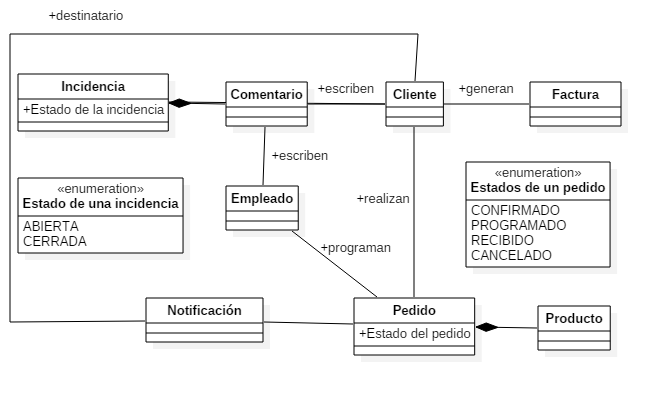
\includegraphics[scale=0.6]{modelo_dominio_final}
\caption{Modelo de dominio del sistema.}
\end{figure}

%%%%%%%%%%%%%%%%%%%%%%%%%%%%%%%%%%%%%%%%%%%%%%%%%%%%%%%%%%%%%%%%%%%%%%%%%%%%%%%
%                       Proceso de desarrollo
%
%%%%%%%%%%%%%%%%%%%%%%%%%%%%%%%%%%%%%%%%%%%%%%%%%%%%%%%%%%%%%%%%%%%%%%%%%%%%%%%

\chapter{Proceso de desarrollo}

\section{Plan de trabajo} \label{sct:PlanTrabajo}

El sistema a implementar se puede dividir en dos partes: front-end y back-end. En lo referente al back-end, este se va a implementar siguiendo dos arquitecturas distintas: una monolítica y otra basada en microservicios. Existirá una gran cantidad de código compartido entre ambas soluciones y las mayores diferencias entre ellas serán las relacionadas con la organización del código. Por este motivo, primero se va a implementar la solución monolítica y una vez implementada se creará una nueva solución donde se refactorizará el código siguiendo los principios que en la sección \ref{sct:FaseDiseño} \nameref{sct:FaseDiseño} se han mencionado.

En cuanto al front-end, las llamadas a la parte servidora van a realizarse a través de invocaciones HTTP. Por tanto, va a estar desacoplado de la implementación que elijamos para el back-end y va a poder emplearse la misma solución para comunicarse con ambas soluciones.

%TODO Incluir un cronograma.

\section{Organización del trabajo}

%%%%%%%%%%%%%%%%%%%%%%%%%%%%%%%%%%%%%%%%%%%%%%%%%%%%%%%%%%%%%%%%%%%%%%%%%%%%%%%
%                       MONOLITICA
%
%%%%%%%%%%%%%%%%%%%%%%%%%%%%%%%%%%%%%%%%%%%%%%%%%%%%%%%%%%%%%%%%%%%%%%%%%%%%%%%

\chapter{Diseño e implementación de la solución monolítica}

\section{Diseño de la solución} \label{sct:DiseñoMonolitico}

A nivel arquitectónico, la aplicación monolítica va a seguir una arquitectura de 6 capas, que detallamos a continuación:

\begin{itemize}

\item \textbf{Capa de contratos}: en esta capa se situarán las interfaces que contienen todas las acciones del back-end que pueden ser invocadas desde el exterior a través de la API. Estas interfaces se implementarán tanto en las capas de Aplicación, Servicios y Proxy. 

También se situarán en esta capa los objetos para la transferencia de datos (DTO). Los DTOs se emplean para desacoplar los servicios que ofrece una API de la representación interna que da el sistema a sus entidades. En lugar de devolver al cliente una entidad tal y como se almacena en base de datos, los DTOs representan una entidad ocultando aquellas propiedades que no necesitan ser transferidas o cambian su formato para que sea más cómodo para el cliente su procesamiento. \footnote{ Crear objetos de transferencia de datos (DTO): https://docs.microsoft.com/es-es/aspnet/web-api/overview/data/using-web-api-with-entity-framework/part-5}

\item \textbf{Capa de aplicación}: en esta capa es donde se implementa la lógica de la parte servidora. Aquí se da implementación a las interfaces que se sitúan en la capa de contratos. Es en esta capa donde se validan los permisos de un usuario que ha realizado una petición al servidor sobre la acción que desea realizar. En caso de que se trate de hacer una operación no válida será esta capa la encarga de lanzar la excepción oportuna. También aquí se situarán los conversores para transformar una entididad en un DTO, que se emplearán principalmente en las operaciones CRUD.

\item \textbf{Capa de servicios}: contiene el punto de entrada del proceso que representa al back-end (el método Main). En esta capa se encuentran los controladores, donde se definen todas las acciones de la API. Cada acción se define a través de un verbo HTTP, la URL donde se localiza y sus parámetros obtenidos a partir del cuerpo o las cabeceras de una petición. La capa de servicios delega en la capa de aplicación para devolver un resultado a cada una de las peticiones que atiende. \footnote{ Control de solicitudes con controladores en ASP.NET Core MVC: https://docs.microsoft.com/es-ES/aspnet/core/mvc/controllers/actions?view=aspnetcore-2.1}

\item \textbf{Capa de dominio}: contiene las entidades del dominio del sistema junto con sus propiedades y los estados asociados a estas. Esta capa es referenciada tanto por la capa de aplicación como por la capa de persistencia.

\item \textbf{Capa de persistencia}: la capa de persistencia ofrece operaciones CRUD para cada una de las entidades que se almacenan en BD a través objetos para el acceso a datos (DAO). La capa de persistencia no trabaja con DTOs: cuando la capa de aplicación le solicita una entidad la devuelve completa y es la capa de aplicación quien a través de los conversores la transforma en un DTO para devolver una representación de la entidad al usuario.

\item \textbf{Capa de proxy}: esta capa contiene clientes necesarios para invocar al back-end a través de llamadas HTTP realizadas por código C\#. Esta capa será referenciada por el front-end a través de un paquete NuGet para comunicar con el back-end. El front-end es quien ejecutará el código contenido en esta capa: cuando se desee comunicar con la parte servidor, en el proceso del front-end se invocará al proxy para realizar una llamada HTTP al back-end. Como debe ofrecer todas las operaciones de la API, implementa las interfaces de la capa de contratos.

\end{itemize}

\begin{figure}[h]
\centering
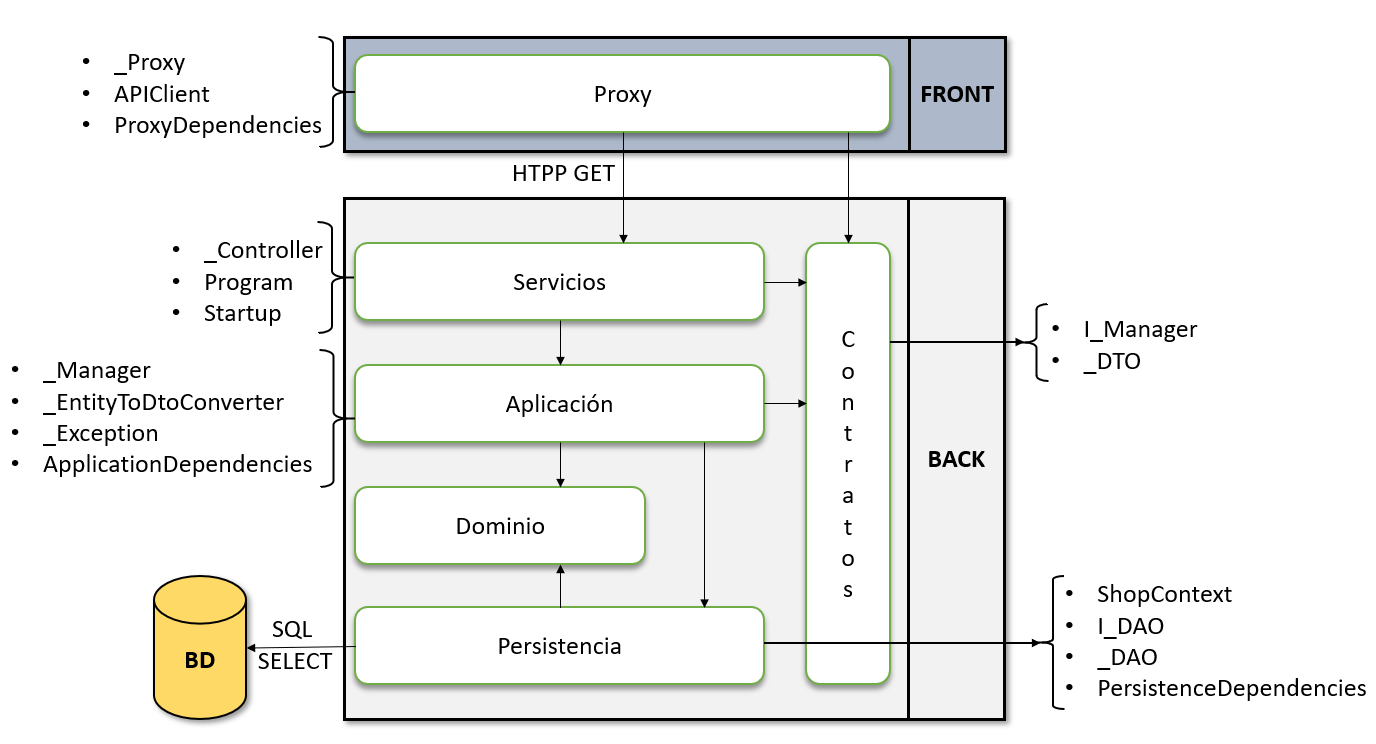
\includegraphics[scale=0.5]{capas}
\caption{Capas del back-end monolítico.}
\end{figure}

A nivel de la solución en Visual Studio, cada capa consistirá en un proyecto distinto. Un proyecto consiste en un archivo XML con extensión *.csproj que tiene una plataforma y dependencias específicas y que se puede compilar de forma independiente. Cada proyecto es un contenedor que organiza sus clases y otros archivos de forma jerárquica. \footnote{ Soluciones y proyectos en Visual Studio: https://docs.microsoft.com/es-es/visualstudio/ide/solutions-and-projects-in-visual-studio} Adicionalmente, existe un proyecto que contiene las pruebas del sistema. Todos los proyectos son .NET Standard 2.0 salvo los de las capa de servicios y pruebas, cuya plataforma es .NET Core 2.1 porque no son librerías y pueden ser ejecutados.

\begin{figure}[h]
\centering
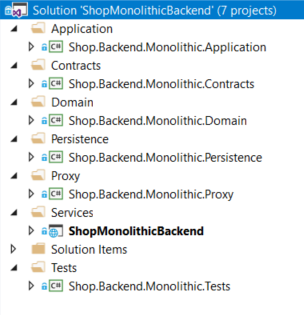
\includegraphics[scale=0.8]{MonolithicSolution}
\caption{Solución del sistema monolítico.}
\end{figure}

A nivel de diseño, se van a definir las siguientes entidades en la capa de dominio: pedido (Order), producto (Product), compra (Purchase), incidencia (Incidence) y comentario (Comment). Estas entidades se pueden obtener a partir del modelo de dominio. Sin embargo, algunos conceptos que aparecen en el modelo de dominio como los informes o las notificaciones no vamos a modelarlas como entidades. No son entidades como tal porque no necesitamos almacenarlas o ofrecer operaciones CRUD sobre ellas, así que vamos a modelarlas como acciones. Simplemente ofreceremos métodos para generar un informe (GenerateReport) y enviar notificaciones (SendNotification).

La relación que existe entre un pedido y un producto es de muchos a muchos: un pedido está formado por múltiples productos y un producto puede estar incluido en diferentes pedidos. Además, la relación cuenta con una propiedad que es el número de unidades del producto en el pedido, que se puede modelar como una clase asociación. Si razonamos a nivel de base de datos, la clase asociación se implementará como una tabla intermedia entre las tablas de pedidos y productos. En nuestro código también lo modelaremos así para emplear la librería de Entity Framework para el mapeo objeto-relacional (ORM).

Con todo esto, el diagrama de clases que se encuentran en la capa de dominio será el siguiente:

\begin{figure}[h]
\centering
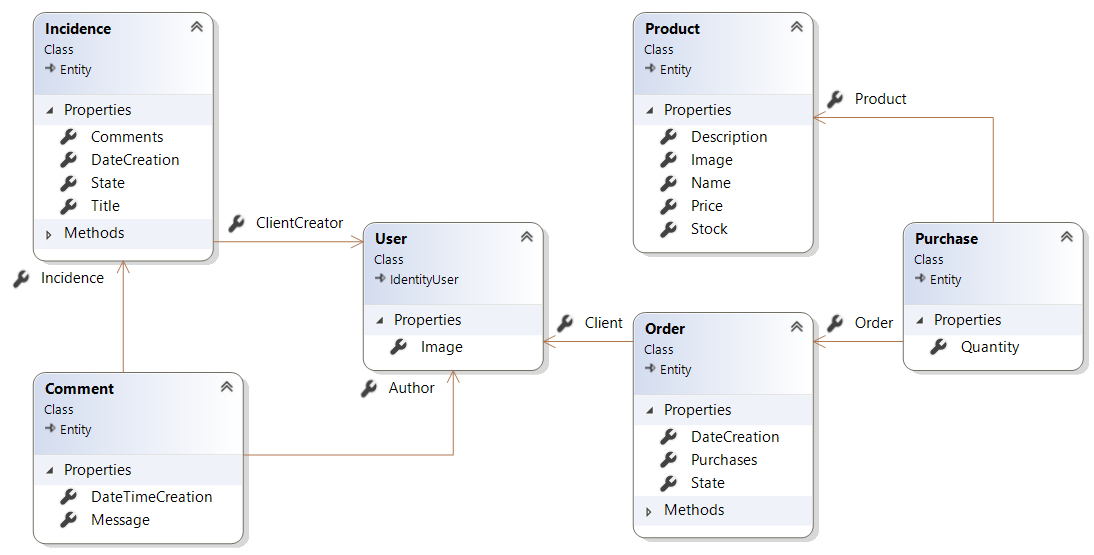
\includegraphics[scale=0.65]{ClassDiagram}
\caption{Diagrama de clases de dominio de la solución monolítica.}
\end{figure}

%%%%%%%%%%%%%%%%%%%%%%%%%%%
% SALTO DE PAGINA
%%%%%%%%%%%%%%%%%%%%%%%%%%%
\newpage

\section{Detalles de la implementación back-end}

\subsection{Operaciones CRUD} \label{subsect:CRUD}

Para la mayoría de entidades que hemos modelado vamos a ofrecer operaciones CRUD. Esto se hará a través de las interfaces que expone la parte servidora en la capa de contratos. Con este propósito vamos a definir una interfaz que exponga estas de forma unitaria y agregada. En los servicios, las operaciones agregadas son un mecanismo para evitar que dos componentes tengan que comunicarse continuamente. Si se tienen que crear una colección de entidades, en lugar de crear una petición al servidor para cada entidad, se envía una única petición con toda la colección. \cite{Newman2015a} 

\begin{figure}[h]
\centering
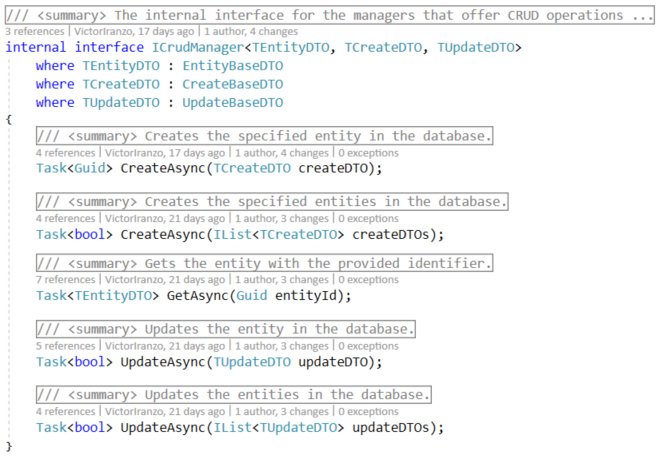
\includegraphics[scale=0.8]{ICrudManager}
\caption{Interfaz interna para las operaciones CRUD.}
\end{figure}

La interfaz es interna porque no debe ser visible fuera de la solución del back-end. Además, es genérica: se define en base a DTOs con diferentes propósitos. Para la creación de una entidad son necesarias solo algunas propiedades y otras como la fecha de creación son calculadas por el sistema y no deben ser provistas en el \textbf{CreateDTO} de la petición. Lo mismo ocurre con la lectura y la actualización de una entidad. Por ejemplo, de una entidad algunas propiedades no está permitido actualizarlas, por lo que no deben incluirse estas en el \textbf{UpdateDTO} de la entidad. 

Sin embargo, no se van a definir únicamente operaciones CRUD para una entidad. Cada entidad tiene una serie de operaciones asociadas, como puede ser generar la factura de un pedido o obtener la lista de incidencias de un usuario. Tanto estas acciones como las CRUD se definen en la interfaz de contratos de la entidad. Si para una entidad se quieren exponer operaciones CRUD, se deben definir los DTOs específicos para las operaciones de lectura, escritura y actualización y se debe extender la interfaz genérica.

\begin{figure}[h]
\centering
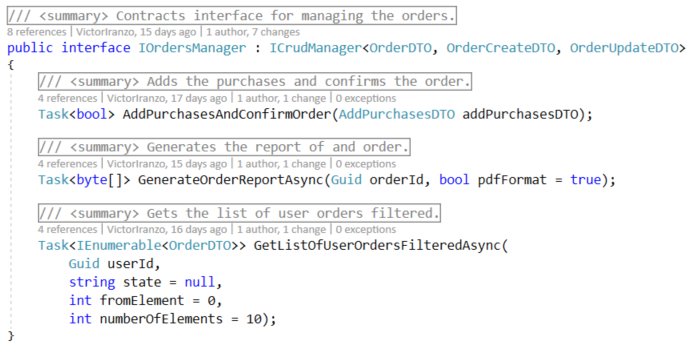
\includegraphics[scale=0.8]{IOrdersManager}
\caption{Interfaz en la capa de contratos asociada a la entidad Pedido.}
\end{figure}

La implementación de las operaciones CRUD en la capa de aplicación también se realizará de forma genérica. Si la implementación de una de las operaciones no se ajusta a la que una entidad necesita, esta puede ser sobreescrita en el manager de la entidad.

Por último, algunas entidades en lugar de ofrecer operaciones CRUD solo ofrecen \textbf{operaciones CUD} (crear, actualizar y eliminar). Estas entidades son las de Comentario y Compra porque podemos considerarlas como secundarias. No tiene sentido exponer un método en la interfaz de back-end para leer un único comentario o obtener el número de unidades de un producto en un pedido. No obstante, si que tiene sentido exponer un método para, por ejemplo, crear o eliminar un comentario dentro de una incidencia. Las operaciones de lectura de estas entidades se realizan a través de la entidad principal asociada. Por ejemplo, cuando solicitamos una incidencia obtendremos todos los comentarios que en la incidencia se han hecho aunque sea una entidad independiente.

\subsection{Seguridad}
%TODO Ha faltado mencionar registro en la clase PersistenceDependencies.
% https://auth0.com/blog/securing-asp-dot-net-core-2-applications-with-jwts/
% https://docs.microsoft.com/es-es/aspnet/core/security/authorization/roles?view=aspnetcore-2.1
% https://docs.microsoft.com/es-es/aspnet/core/security/authorization/simple?view=aspnetcore-2.1
% https://docs.microsoft.com/es-es/aspnet/core/security/authentication/identity?view=aspnetcore-2.1&tabs=visual-studio%2Caspnetcore2x

La mayoría de métodos expuestos en la API del backend requieren de mecanismos de autorización para establecer si la persona que realiza una petición puede acceder o no a los datos que solicita. Con este propósito, vamos a hacer uso de \textbf{ASP.NET Core Identity} y de tokens de seguridad JWT (JSON Web Token). 

Identity es el sistema de ASP.NET Core para administrar los usuarios registrados de una aplicación a través de proveedores externos como Google y Facebook o a través de una base de datos de usuarios propia. \footnote{ Introducción a la identidad en ASP.NET Core: https://docs.microsoft.com/es-es/aspnet/core/security/authentication/identity} Atendiendo a los requisitos especificados, no necesitamos que nuestros usuarios se puedan autenticar a través de proveedores externos, por lo que vamos a optar por gestionar los usuarios de la aplicación nosotros mismos. Los pasos para conseguirlo se resumen a continuación:

\begin{itemize}

\item En la capa de dominio, se debe crear una entidad que represente al usuario de la aplicación y que herede de la clase IdentityUser. La clase IdentityUser provee numerosos atributos, como el nombre o el correo electrónico. Se puede añadir cualquier atributo más asociado al usuario de la aplicación dentro de la clase User.

\begin{figure}[h]
\centering
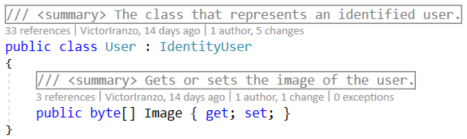
\includegraphics[scale=0.8]{User}
\caption{La clase User.}
\end{figure}

\item En la capa de persistencia, para asegurar la creación de las tablas asociadas a Identity, el contexto de la aplicación que representa a la base de datos debe extender la clase IdentityDbContext<User>. En la base de datos, las tablas de datos creadas automáticamente por Identity se identifican por el prefijo AspNet.

\begin{figure}[h]
\centering
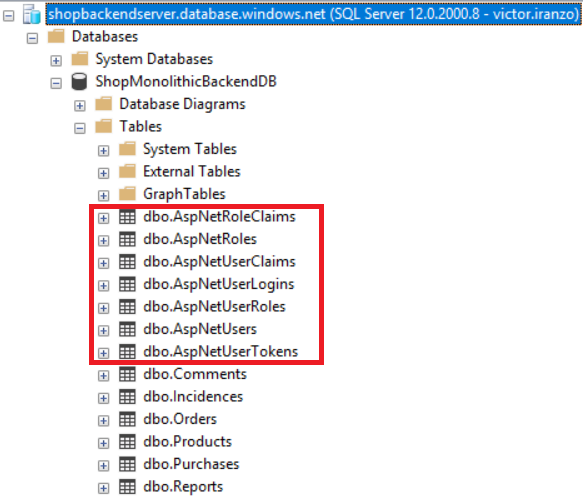
\includegraphics[scale=0.8]{BDMonolitica}
\caption{Tablas creadas por ASP.NET Core Identity.}
\end{figure}

\item En la capa de servicios, a los métodos de la API que requieran de autorización se les ha de añadir el atributo Authorize. Con esto, cuando se realice una petición sin proveer un token de autorización se devolverá automáticamente un error 401: Unauthorized. En el atributo Authorize se puede especificar si el método puede ser ejecutado solo por los usuarios que tengan cierto rol. \footnote{ Autorización basada en roles en ASP.NET Core: https://docs.microsoft.com/es-es/aspnet/core/security/authorization/roles?view=aspnetcore-2.1} Por ejemplo, podemos establecer que las operaciones agregadas de tipo CRUD solo puedan ser invocadas por los usuarios con el rol Administrador.

\begin{figure}[h]
\centering
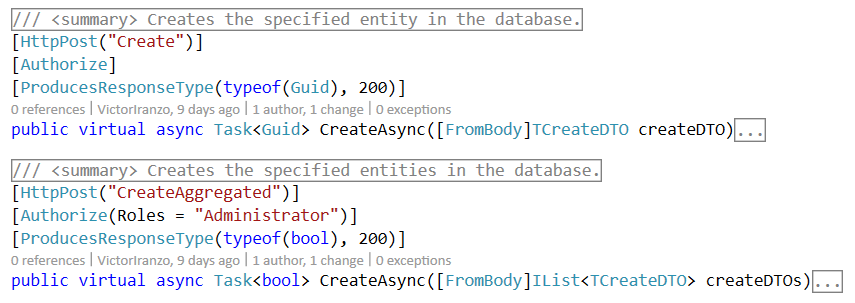
\includegraphics[scale=0.7]{Authorize}
\caption{Ejemplo de métodos de la clase de servicios.}
\end{figure}

\item Por último, en la capa de servicios se debe especificar que el mecanismo por el cual el usuario proveerá su identidad será a través de tokens JWT. Para ello, en la clase Startup se debe añadir a la colección de servicios el servicio de autenticación con este tipo de tokens, indicando que los únicos tokens válidos son los firmados con la clave provista en el archivo de configuración. \footnote{ Securing ASP.NET Core 2.0 Applications with JWTs: https://auth0.com/blog/securing-asp-dot-net-core-2-applications-with-jwts/}

\begin{figure}[h]
\centering
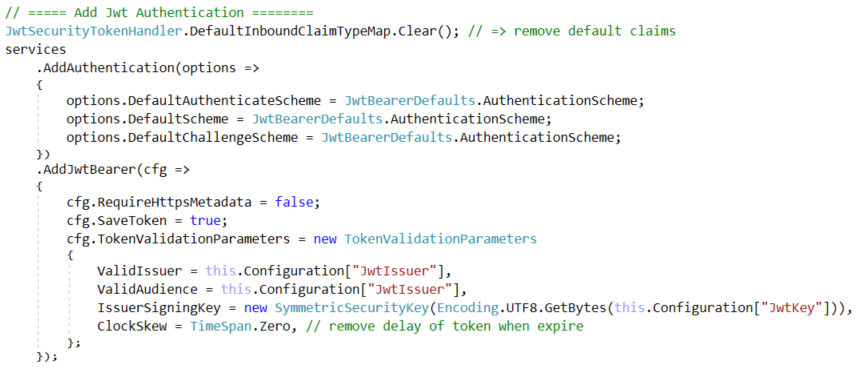
\includegraphics[scale=0.7]{jwt}
\caption{Pieza de código para añadir la autenticación usando tokens JWT.}
\end{figure}

\end{itemize}

El usuario podrá obtener el token que le identifica a través del método Login del manager de Seguridad. Para hacerlo, deberá proveer su correo electrónico y contraseña. En la implementación de este método en la capa de aplicación se comprueba que el correo electrónico y contraseña coinciden con los almacenados en las tablas de Identity. Si coinciden, el método devuelve un token JWT donde se incluirán los datos del usuario y la fecha en la que el token expira. En cada petición HTTP que haga el usuario a la parte servidora deberá proveer este en la cabecera.

\begin{figure}[h]
\centering
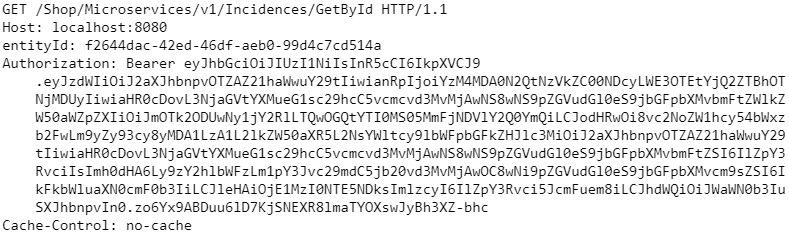
\includegraphics[scale=0.8]{http}
\caption{Ejemplo de petición HTTP donde se incluye un token de seguridad.}
\end{figure}

%%%%%%%%%%%%%%%%%%%%%%%%%%%
% SALTO DE PAGINA
%%%%%%%%%%%%%%%%%%%%%%%%%%%
\newpage

\subsection{Persistencia} \label{subsect:Persistencia}

Para la persistencia se va a emplear \textbf{Entity Framework Core} para el mapeo objeto-relacional y una base de datos SQL en la nube de \textbf{Microsoft Azure}. Entity Framework Core es una versión multiplataforma del ORM Entity Framework (EF) para trabajar con una base de datos mediante objetos .NET. \footnote{Descripción general de Entity Framework Core: https://docs.microsoft.com/es-es/ef/core/}

Vamos a emplear una aproximación Code-First para el diseño de la base de datos. Esta aproximación nos permite diseñar primero las entidades de nuestro dominio a través de las clases en la capa de dominio y luego trasladar sus atributos y relaciones a un esquema de base de datos gracias a EF. \footnote{What is Code-First?: http://www.entityframeworktutorial.net/code-first/what-is-code-first.aspx}

Para la creación de la base de datos se debe ir al portal de Azure \footnote{ Portal de Azure: https://portal.azure.com/} y navegar hasta la página SQL Databases. Para la creación de la base de datos hay que proveer principalmente su nombre, la suscripción a la que se redirigirán los costes asociados, el grupo de recursos en el que se incluirá y el servidor donde se emplazará.

\begin{figure}[h]
\centering
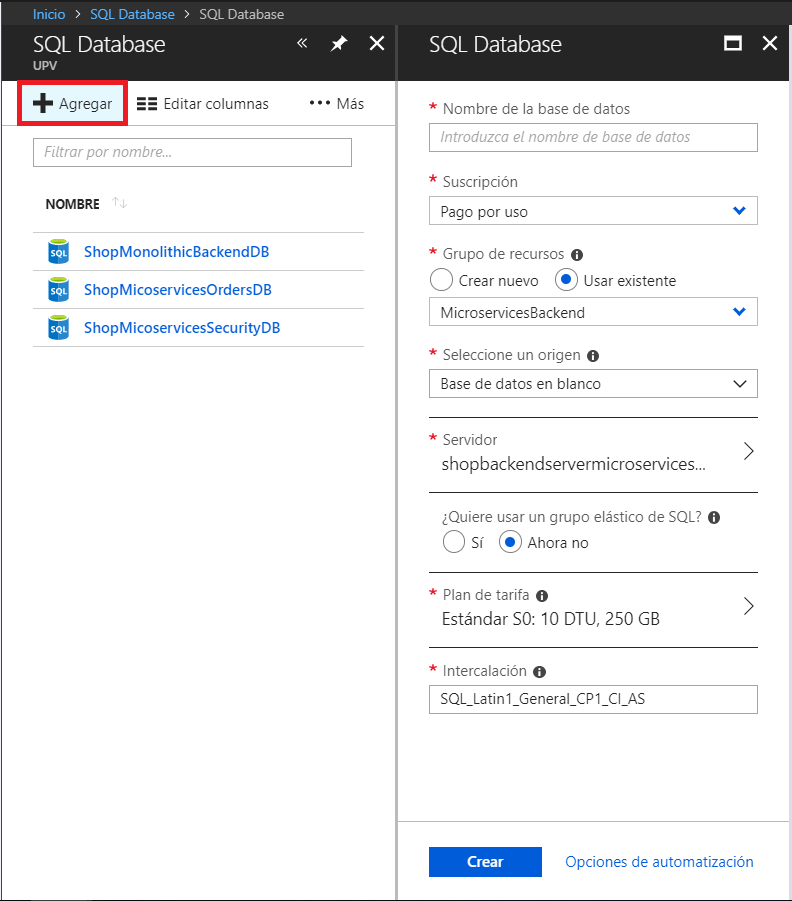
\includegraphics[scale=0.4]{CreateDB}
\caption{Creación de una base de datos SQL en Azure.}
\end{figure}

Una vez creada, debemos ir al recurso y en la pestaña de cadenas de conexión copiar la asociada a .NET. La cadena de conexión la pegaremos en el archivo de configuración de la capa de servicios. En la clase Startup del mismo proyecto leeremos la cadena de conexión para configurar la clase ShopContext.

\begin{figure}[h]
\centering
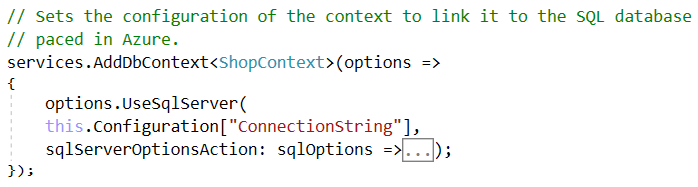
\includegraphics[scale=0.7]{AddDbContext}
\caption{Configuración del contexto de la capa de persistencia para apuntar a la BD en Azure.}
\end{figure}

En la clase ShopContext debemos indicar cuáles son las entidades del dominio que se añadirán como tablas a la BD. Para cada entidad del dominio se creará un DbSet distinto.

\begin{figure}[h]
\centering
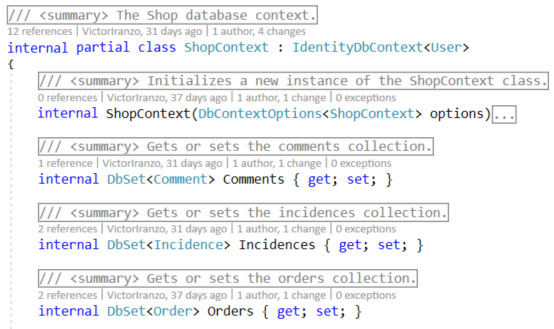
\includegraphics[scale=0.8]{ShopContext}
\caption{Clase ShopContext.}
\end{figure}

Por último, para que desde otras capas accedan a los datos emplearemos el \textbf{patrón DAO}. Exponer el contexto entero fuera de la capa de persistencia puede ser peligroso porque permitiría modificar desde otras capas aspectos que solo deben conocerse en esta capa. Por ello, se definirá para cada entidad del dominio una interfaz para acceder a sus datos donde las operaciones permitidas están acotadas. De nuevo, tanto estas interfaces como su implementación se pueden definir de forma genérica y si se desea se puede extender o sobreescribir su comportamiento.

\begin{figure}[h]
\centering
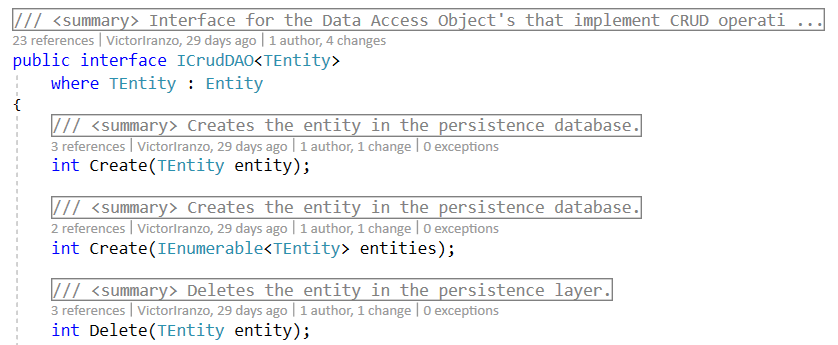
\includegraphics[scale=0.8]{ICrudDAO}
\caption{Interfaz genérica para los DAOs que exponen operaciones CRUD.}
\end{figure}

\subsection{Informes empleando la librería Open XML PowerTools}

La generación de informes es una de las funcionalidades más empleadas en los software de gestión. En los requisitos de nuestro sistema solo se ha establecido un informe: la factura de un pedido. Esto no implica que debamos dejar de seguir el principio de responsabilidad única. La lógica para generar un informe debe ser genérica para que no dependa del tipo de informe que se va a generar y así pueda ser invocada desde diferentes sitios. Vamos a hacer uso de una librería para la generación de informes con estas librerías: \textbf{Open XML PowerTools}.

Open XML PowerTools provee funcionalidades para la combinación de documentos, la conversión de estos a diferentes formatos y la creación de informes a partir de plantillas. \footnote{ Página de GitHub de Open XML PowerTools: https://github.com/OfficeDev/Open-Xml-PowerTools}. Para generar un informe se separan explícitamente los datos que lo originan y la plantilla del documento. En las plantillas se define cómo se van a renderizar los datos mediante un lenguaje basado en anotaciones. Este lenguaje nos permite renderizar contenido en base a condiciones, iterar sobre las colecciones en los datos, crear tablas, etc.

\begin{figure}[h]
\centering
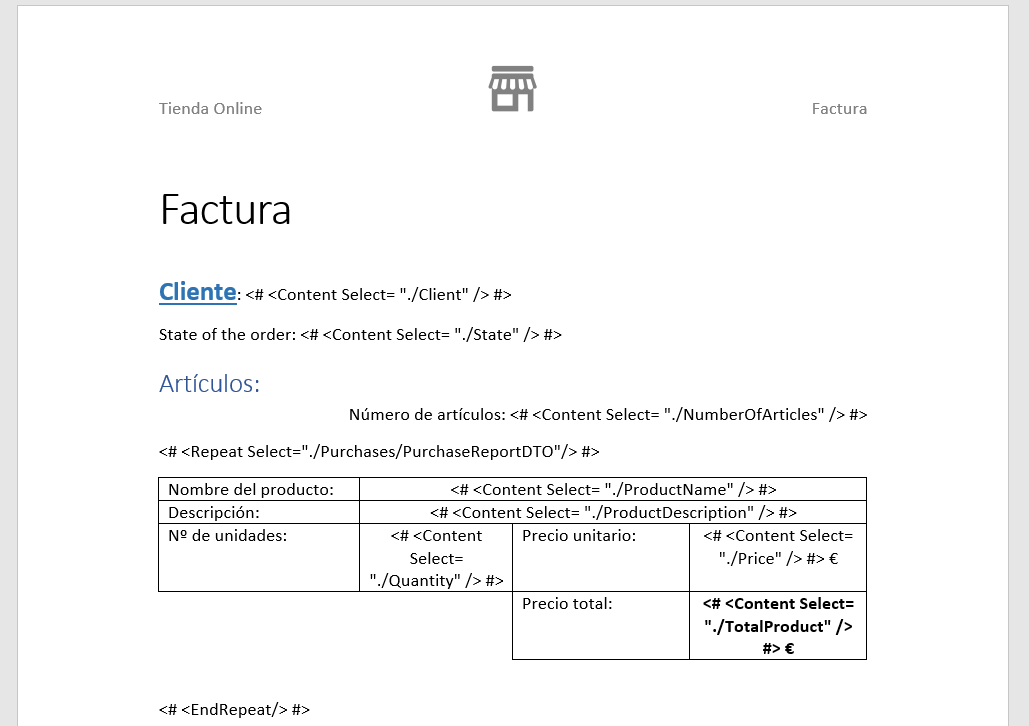
\includegraphics[scale=0.5]{Factura}
\caption{Plantilla para la creación de facturas.}
\end{figure}

Las plantillas se almacenarán en la base de datos y cuando se quiera generar un informe se recuperará esta para ensamblar el informe. Los métodos para generar un informe concreto estarán expuestos en los managers de la entidad asociada al informe. Por ejemplo, el método para generar la factura de un pedido se situará en el OrdersManager. En este método se recuperarán los datos para generar la factura y se enviarán estos al manager de informes para que los combine con la plantilla de la factura.

\subsection{Notificaciones con la librería MailKit}

Con las notificaciones ocurre lo mismo que con los informes: solo existe un caso de uso que envíe una notificación al cliente, pero para segregar responsabilidades vamos a crear un manager específico para este propósito. Para enviar notificaciones se va emplear la librería \textbf{MailKit}, una librería multiplataforma con utilidades sobre los protocolos IMAP, POP3 y SMTP.

Para desacoplar los mensajes a enviar y el código para enviarlo se hará uso de un DTO que contenga el usuario destinatario, el asunto del correo y el cuerpo del mismo. Tanto el cuerpo como el asunto de la notificación se definirán en archivos de recursos en la capa de aplicación.

\begin{figure}[h]
\centering
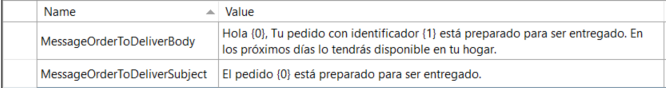
\includegraphics[scale=1]{NotificationsMessage}
\caption{Archivo de recursos para las notificaciones.}
\end{figure}

\subsection{Inyección de dependencias}

La \textbf{inyección de dependencias} (DI) es un mecanismo para desacoplar un objeto de sus colaboradores. En lugar de instanciar o obtener una referencia a los objetos de los que depende una clase, estos se declaran en el constructor de la clase y es el sistema quien automáticamente los resuelve e instancia. \footnote{ Inserción de dependencias en ASP.NET Core: https://docs.microsoft.com/es-es/aspnet/core/fundamentals/dependency-injection} 

\begin{figure}[h]
\centering
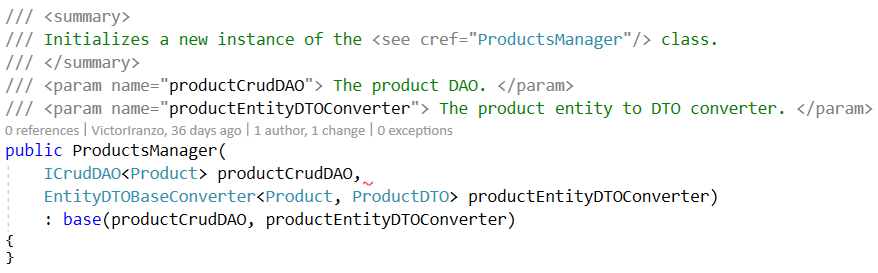
\includegraphics[scale=0.8]{ProductsManager}
\caption{Constructor de la clase ProductsManager donde se aplica DI.}
\end{figure}

El uso de interfaces reduce el acoplamiento entre la definición de las operaciones de una clase y las implementaciones concretas que esta definición puede tener. Sin embargo, es necesario indicar con qué implementación se resuelve una interfaz cuando esta se inyecta en el constructor de una clase. Para ellos, se emplean una serie de métodos sobre la colección de servicios donde el sistema busca sus dependencias para indicar cómo resolver cada interfaz. El método más empleado es AddScoped. Este método instancia el objeto de la dependencia una vez por cada petición que el servidor recibe y comparte este mismo objeto entre todas las clases que dependan de él.

En nuestra solución, cada capa es responsable de registrar las diferentes interfaces que contiene junto con la clase que la implementa. De esta forma, desde otras capas se podrán emplear las interfaces resultas.

\begin{figure}[h]
\centering
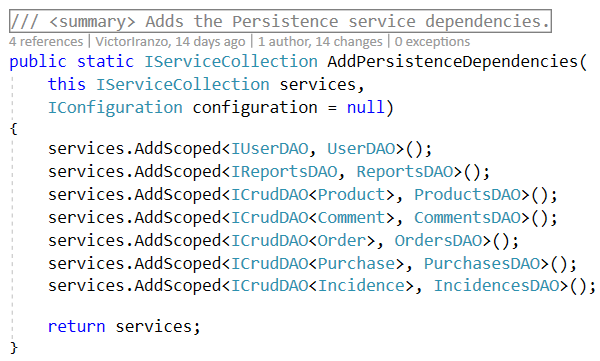
\includegraphics[scale=0.9]{ResolucionDependencias}
\caption{Registro de interfaces en la capa de persistencia.}
\end{figure}

\subsection{Documentando la API con Swagger UI}

\textbf{Swagger} es un conjunto de herramientas de código abierto para describir la estructura de una API, crear clientes para consumirla en diferentes lenguajes (Swagger CodeGen) y documentarla para que los usuarios puedan emplearla de forma interactiva (Swagger UI). \footnote{ Documentación oficial de Swagger: https://swagger.io/docs/specification/2-0/what-is-swagger/}

En este apartado nos centraremos en la construcción de la API interactiva. Para hacerlo, basta con añadir la siguiente pieza de código en la clase Startup de la capa de servicios. Aparte de proveer algunos metadatos como la versión de la API o su mantenedor, se debe indicar que los controladores para generar la documentación se encuentran en el ensamblado actual.

\begin{figure}[h]
\centering
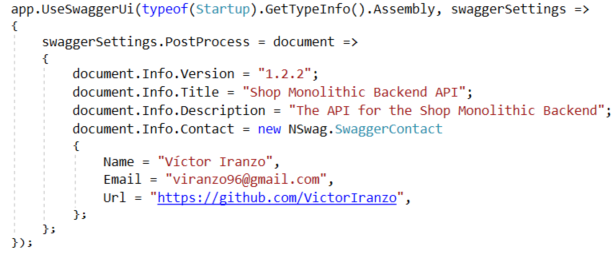
\includegraphics[scale=0.9]{SwaggerUI}
\caption{Metadatos de la API especificados en la clase Startup.}
\end{figure}

La documentación de la API se genera en la dirección formada por la unión de la URL del servidor y el recurso con nombre swagger. Para generar la documentación de los métodos, Swagger hace uso de la documentación del método del controlador de la capa de servicios que la origina. En la documentación de cada método se incluye información como la descripción de los parámetros o el tipo de respuesta que da el método.

\begin{figure}[h]
\centering
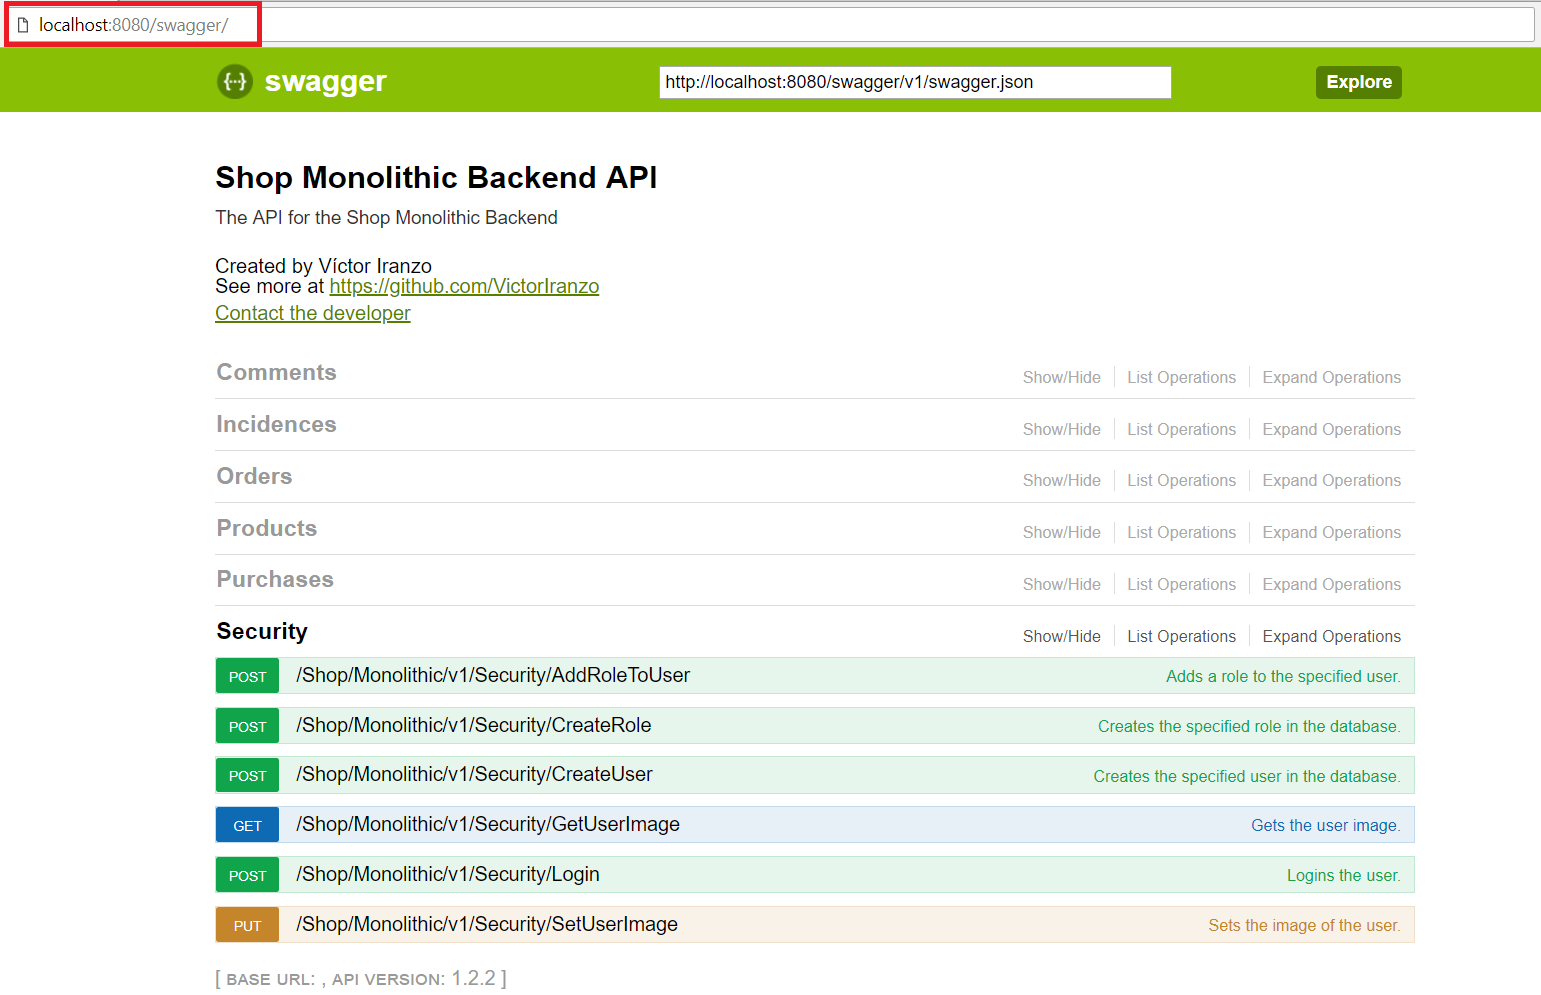
\includegraphics[scale=0.4]{SwaggerAPI}
\caption{Documentación de la API generada con Swagger UI.}
\end{figure}

\subsection{Logging}
%TODO Decidir si eliminarlo.
En el entorno de desarrollo puede ser útil emplear logs que capturen todo lo que sucede en el proceso del servidor. Para hacerlo, simplemente se deben añadir las siguientes líneas de código en la clase Startup de la capa de servicios.

\begin{figure}[h]
\centering
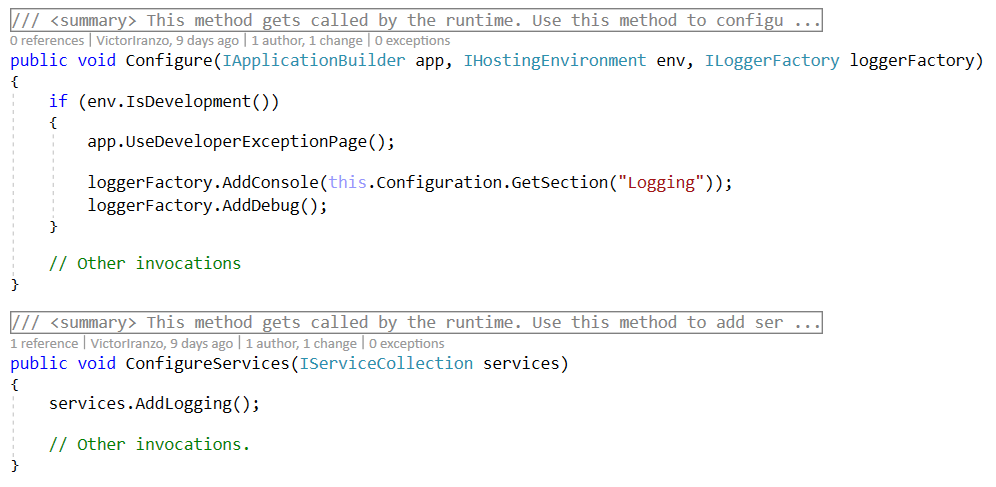
\includegraphics[scale=0.7]{loggingDev}
\caption{Añadir servicios para el logging.}
\end{figure}

Información como el entorno donde se ejecuta el servidor, las peticiones HTTP que se realicen al servidor o las consultas a base de datos quedarán registrados en la consola del proceso.

\begin{figure}[h]
\centering
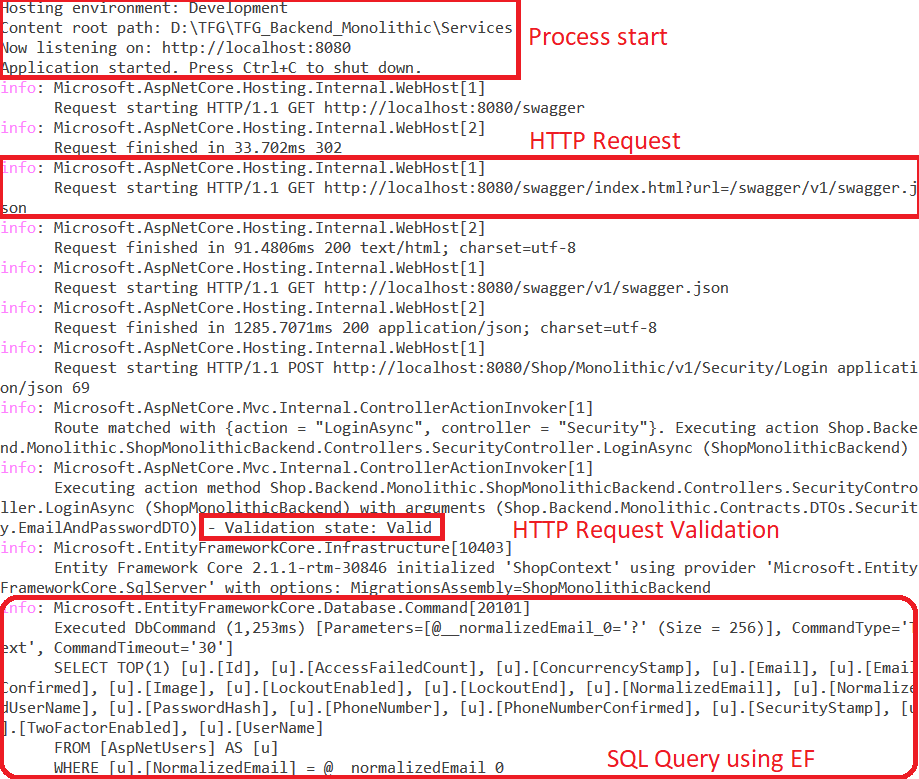
\includegraphics[scale=0.5]{logging}
\caption{Ejemplo del contenido de un log.}
\end{figure}

\subsection{Generación de la capa de proxy}
%TODO Incluir algo más de NSwag.

Como hemos comentado en la sección \ref{sct:DiseñoMonolitico} \nameref{sct:DiseñoMonolitico}, la capa de proxy se emplea para invocar a la API de la parte servidora a través de llamadas HTTP. Para cada una de las interfaces de contratos vamos a crear un proxy, que implementará sus métodos delegando en un cliente HTTP generado automáticamente con \textbf{NSwag}. NSwag es un conjunto de herramientas para varias plataformas, entre ellas .NET Core, para la generación de especificaciones Swagger a partir de los controladores definidos en C\# y la generación de clientes HTTP para el consumo de estos controladores. \footnote{ Página de GitHub de NSwag: https://github.com/RSuter/NSwag} \footnote{ NSwag Tutorial: How to integrate NSwag into your ASP.NET Core Web API project: https://www.youtube.com/watch?v=lF9ZZ8p2Ciw}

El cliente HTTP autogenerado es inyectado en el proxy a través del constructor. El proxy también es el encargado de adaptar los parámetros de la interfaz de contratos a los parámetros que espera el cliente HTTP. Esta adaptación es necesaria porque, por ejemplo, en las peticiones HTTP para los métodos GET no se puede especificar un Body y todos los parámetros se deben pasar a través de la cabecera de la petición. Como consecuencia, los parámetros solo pueden ser de tipos simples como una cadena (string) y objetos muy empleados como los identificadores (Guid) han de ser transformados a tipos más simples.

\begin{figure}[h]
\centering
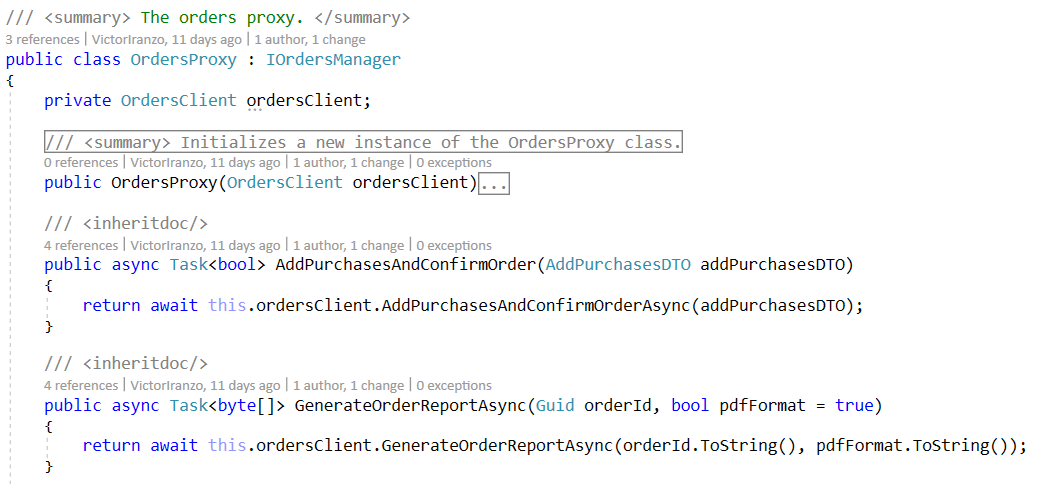
\includegraphics[scale=0.7]{OrdersProxy}
\caption{Fragmento del proxy de pedidos donde se adaptan los parámetros a tipos simples.}
\end{figure}

\subsection{Calidad del código}

Para asegurar la calidad del código se ha hecho uso de dos herramientas: CodeMaid y StyleCop.

\begin{itemize}

\item \textbf{CodeMaid}: es una extensión de Visual Studio para la limpieza automática de código C\# y otros lenguajes. En el proceso de limpieza, CodeMaid ordena los métodos y propiedades de acuerdo a los estándares, revisa el formato de los comentarios, elimina las referencias a espacios de nombres que no se emplean, etc. \footnote{ Página oficial de CodeMaid: http://www.codemaid.net/}

\item \textbf{StyleCop}: es un analizador estático de código C\# desarrollado por Microsoft. Se basa en reglas centradas en aspectos como la documentación, la ordenación de los elementos o el estilo de código. Además, permite configurar las reglas que se aplican, definir excepciones a una de ellas o la creación de reglas propias. \footnote{Página de la Wikipedia de StyleCop: https://en.wikipedia.org/wiki/StyleCop} 

En la mayoría de proyectos se ha configurado para que las alertas que devuelve StyleCop cuando no se cumple una regla se trate como un error y no como una alerta. Esto se puede conseguir añadiendo la opción TreatWarningsAsErrors en los archivos .csproj.

\end{itemize}

\begin{figure}[h]
\centering
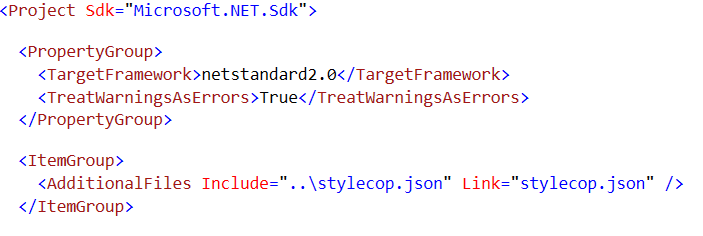
\includegraphics[scale=0.9]{TreatWarning}
\caption{Fragmento de un proyecto donde se añade la opción TreatWarningsAsErrors.}
\end{figure}

\section{Interfaz de usuario}

Como hemos comentado en la sección \ref{sct:PlanTrabajo} \nameref{sct:PlanTrabajo}, vamos a implementar una interfaz de usuario que cumpla con los casos de uso y se pueda emplear para comunicar tanto con la solución monolítica como con la basada en microservicios. Para desacoplar el desarrollo del back-end y el front-end, la aplicación móvil va a desarrollarse en un repositorio de código distinto.

%TODO Decidir si poner esto. https://techcrunch.com/2017/05/11/microsoft-now-lets-ios-developers-deploy-run-and-test-their-apps-directly-from-windows/
La solución de la UI está compuesta por dos proyectos. El primero es en el que se localiza la mayoría del código que se ha implementado, un proyecto .NET Standard con el código compartido por todas las plataformas. El segundo es el proyecto específico para la plataforma Android. Los proyectos asociados a las plataformas UWP y iOS han sido eliminados para hacer más simple su desarrollo.

\begin{figure}[h]
\centering
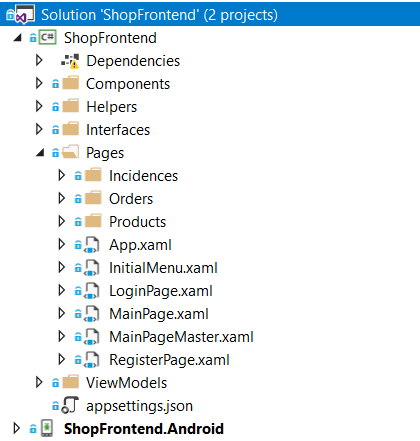
\includegraphics[scale=0.8]{ShopFrontEnd}
\caption{Solución de la interfaz de usuario hecha con Xamarin.Forms.}
\end{figure}

Podemos citar las siguientes características que se desean poner en valor de la implementación de la interfaz de usuario:

\begin{itemize}

\item \textbf{Presentación de resultados de forma paginada}: en el back-end se han implementado diferentes métodos para obtener resultados (como la lista de incidencias de un usuario o la lista de productos) de forma paginada, ordenada y a través de filtros. La paginación en las invocaciones a una API son una forma de mejorar el rendimiento de una aplicación porque evita traer más resultados de los que luego se consultan. El filtrado y la ordenación de los datos están más centrados en mejor la experiencia del usuario (UX).\footnote{ REST API Design: Filtering, Sorting, and Pagination: https://www.moesif.com/blog/technical/api-design/REST-API-Design-Filtering-Sorting-and-Pagination/} 

A nivel de UI se ha implementado de tal forma que se soliciten al back-end una cantidad de datos aproximada a la que se puede mostrar en la pantalla de un dispositivo. Cuando el usuario haga scroll para mostrar más resultados, se realizará una nueva petición en segundo plano a la parte servidora solicitando el siguiente bloque de datos. Mientras se cargan los datos, el usuario visualizará un elemento que indica que el sistema está trabajando en segundo plano para traer más datos.


%TODO Interesante https://msdn.microsoft.com/en-us/magazine/dd419663.aspx https://blogs.msdn.microsoft.com/johngossman/2005/10/08/introduction-to-modelviewviewmodel-pattern-for-building-wpf-apps/
\item \textbf{Uso de ViewModels}: la separación de responsabilidades no es un principio que se deba aplicar solo en el back-end. El patrón arquitectónico \textbf{Model-View-ViewModel} (MVVM) divide la interfaz de usuario en 3 capas: la vista, empleando páginas XAML, los datos tal como se obtienen en su origen, también llamados el modelo, y el modelo de la vista, que conecta ambos y se emplea para rellenar la vista. \footnote{From Data Bindings to MVVM: https://docs.microsoft.com/es-es/xamarin/xamarin-forms/xaml/xaml-basics/data-bindings-to-mvvm} 

La diferencia entre este patrón y otros como el Model-View-Controller(MVC) es que en MVC los datos con los que se llena la vista son los que se obtienen en el origen y es el controlador quien ha de adaptarlos a cómo se visualizan en la vista. En cambio, en MVVM la vista y el modelo de la vista suelen relacionarse a través de enlaces (bindings) en el propio XAML y se notifican mutuamente cuando alguna de sus propiedades cambia. \footnote{ Patterns - WPF Apps With The Model-View-ViewModel Design Pattern: https://msdn.microsoft.com/en-us/magazine/dd419663.aspx}

Sin embargo, usar este patrón puede ser excesivo para UIs muy sencillas. \footnote{Advantages and disadvantages of M-V-VM: https://blogs.msdn.microsoft.com/johngossman/2006/03/04/advantages-and-disadvantages-of-m-v-vm/} Por este motivo, hemos empleado objetos ViewModel en solo aquellos casos que era necesario adaptar los datos del modelo a la vista. Lo que aquí definimos como modelo es un DTO que devuelve la parte servidora y ya está diseñado para que contenga solo la información estrictamente necesaria. Un ejemplo en el que se emplea un ViewModel es el ProductViewModel, donde se tiene que transformar la imagen que se recibe del ProductDTO de byte[] a un ImageSource.

\begin{figure}[h]
\centering
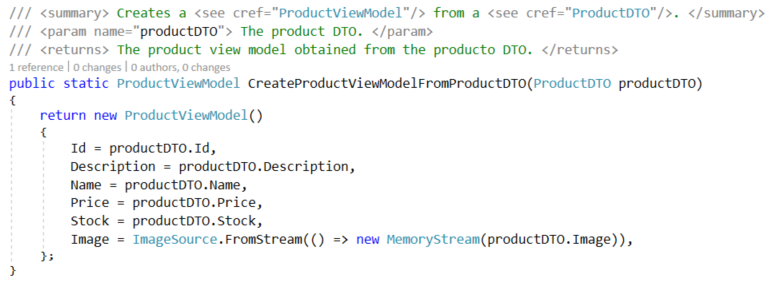
\includegraphics[scale=0.8]{ProductViewModel}
\caption{Método para transformar de un DTO a un modelo de una vista.}
\end{figure}

\item \textbf{Código específico de plataforma}: existen algunos servicios que no se pueden implementar en el proyecto compartido por todas las plataformas. Estos servicios están relacionados con aspectos muy ligados a cada plataforma, como puede ser el sistema de archivos. Para este propósito se define una interfaz en el proyecto compartido. Cada una de las plataformas debe dar una implementación concreta a esta interfaz. Desde el proyecto genérico, se hace uso de la interfaz y será el sistema quien se encargará de dirigir la operación que se invoca sobre la interfaz a la implementación de la plataforma. \footnote{Native Services with Xamarin.Forms? It's DependencyService to the Rescue: https://visualstudiomagazine.com/articles/2015/09/01/native-services-with-xamarinforms.aspx}

\begin{figure}[h]
\centering
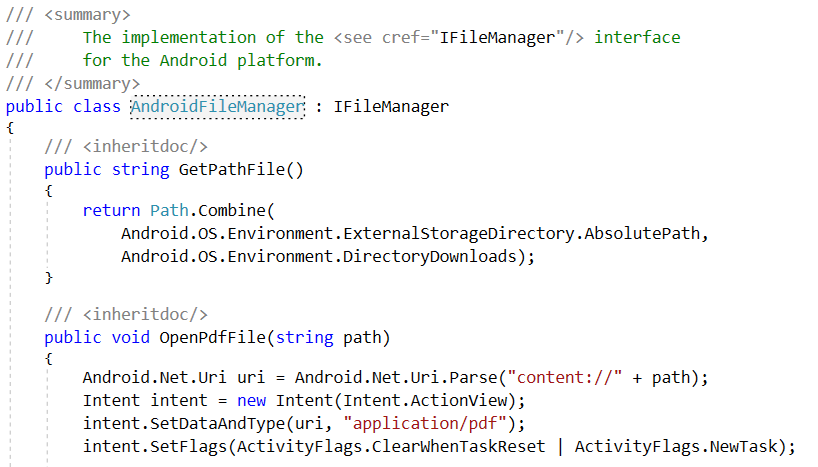
\includegraphics[scale=0.8]{AndroidFileManager}
\caption{Servicio concreto del proyecto de Android.}
\end{figure}

\end{itemize}

Como material adicional, en el apéndice \ref{ch:ModeloNavegacion} \nameref{ch:ModeloNavegacion} se incluyen capturas de la aplicación desarrollada y la navegación que existe entre las diferentes pantallas.

\section{Pruebas}
%TODO Pruebas del CRUD.
- Número de pruebas.
- Pruebas realizadas.
- Captura de las pruebas ejecutadas satisfactoriamente.

\section{Despliegue}

%%%%%%%%%%%%%%%%%%%%%%%%%%%%%%%%%%%%%%%%%%%%%%%%%%%%%%%%%%%%%%%%%%%%%%%%%%%%%%%
%                       MICROSERVICIOS
%
%%%%%%%%%%%%%%%%%%%%%%%%%%%%%%%%%%%%%%%%%%%%%%%%%%%%%%%%%%%%%%%%%%%%%%%%%%%%%%%

\chapter{Diseño e implementación de la solución basada en microservicios}

A lo largo del capítulo anterior nos hemos centrado sobretodo en aspectos de implementación relacionados con diferentes herramientas como Identity o Swagger. En este capítulo nos vamos a centrar más en el diseño ya que, como hemos dicho en el apartado \ref{sct:PlanTrabajo} \nameref{sct:PlanTrabajo}, vamos a refactorizar la solución monolítica y a nivel de código apenas va a verse modificada.

\section{Diseño de la solución}

Para la descomposición de la solución en microservicios vamos a aplicar los principios que hemos explicado en el apartado \ref{sct:FaseDiseño} \nameref{sct:FaseDiseño}. Se tienen que extraer contextos bien delimitados sin importar en un primer momento el tamaño de estos. Aunque contemos con la experiencia del desarrollo de la solución monolítica, el tamaño de los microservicios se puede ajustar más adelante evaluando si vale la pena dividir un microservicio.

Concretamente, para representar visualmente la división en contextos delimitados se va emplear el modelo de dominio del caso de estudio de forma similar a como se ha hecho en la figura \ref{fig:BoundedContexts}. A continuación, detallamos cada uno de ellos, centrándonos en las capacidades que ofrece al negocio y no tanto en las entidades que maneja:

\begin{figure}[h]
\centering
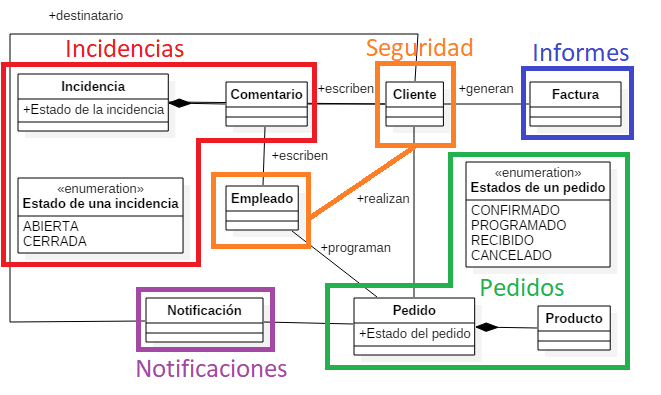
\includegraphics[scale=1]{ShopBoundedContexts}
\caption{División del modelo de dominio en contextos delimitados.}
\end{figure}

\begin{itemize}

\item \textbf{Incidencias}: permite la creación de incidencias, obtener las incidencias de un cliente y añadir comentarios dentro de una incidencia.

\item \textbf{Seguridad}: ofrece las funcionalidades de registro de nuevos clientes y login. Además, persiste los datos de los clientes, por lo que algunos de los microservicios tendrán una referencia a este, por ejemplo, para obtener el cliente o empleado que escribió un comentario.

\item \textbf{Informes}: es un motor que almacena las plantillas de los informes que se pueden generar y simplemente combina esta con los datos que recibe para generar un documento de salida. No ofrece directamente ninguna funcionalidad al cliente: se trata de un \textbf{microservicio interno} que otros servicios emplean.

\item \textbf{Notificaciones}: al igual que el microservicio de informes, no está ligado a ningún tipo de dato. Simplemente, ofrece la funcionalidad de enviar una notificación con el contenido que recibe como parámetro al destinatario especificado. También es un microservicio interno.

\item \textbf{Pedidos}: permite obtener los pedidos de un cliente, generar una factura de un pedido, añadir productos...En este servicio se ha incluido la entidad Producto. Podríamos considerar un microservicio de catálogo al que solo tuvieran acceso los empleados del comercio para gestionar el número de unidades en stock o la creación de nuevos productos. Sin embargo, ninguna funcionalidad fuera del contexto de los pedidos se relaciona con los productos, por lo que la incluiremos en este servicio y más adelante evaluaremos si vale la pena representarla como un microservicio independiente. 

\end{itemize}

\subsection{Arquitectura interna de los microservicios}

En el apartado \ref{subsec:Poliglota} \nameref{subsec:Poliglota} se ha reflexionado sobre que una arquitectura basada en microservicios permite emplear diferentes tecnologías, arquitecturas y bases de datos en cada microservicio. Para validar lo que en este apartado se dice, vamos a desarrollar algunos microservicios con diferentes combinaciones de estas 3 características.

\begin{figure}[h]
\centering
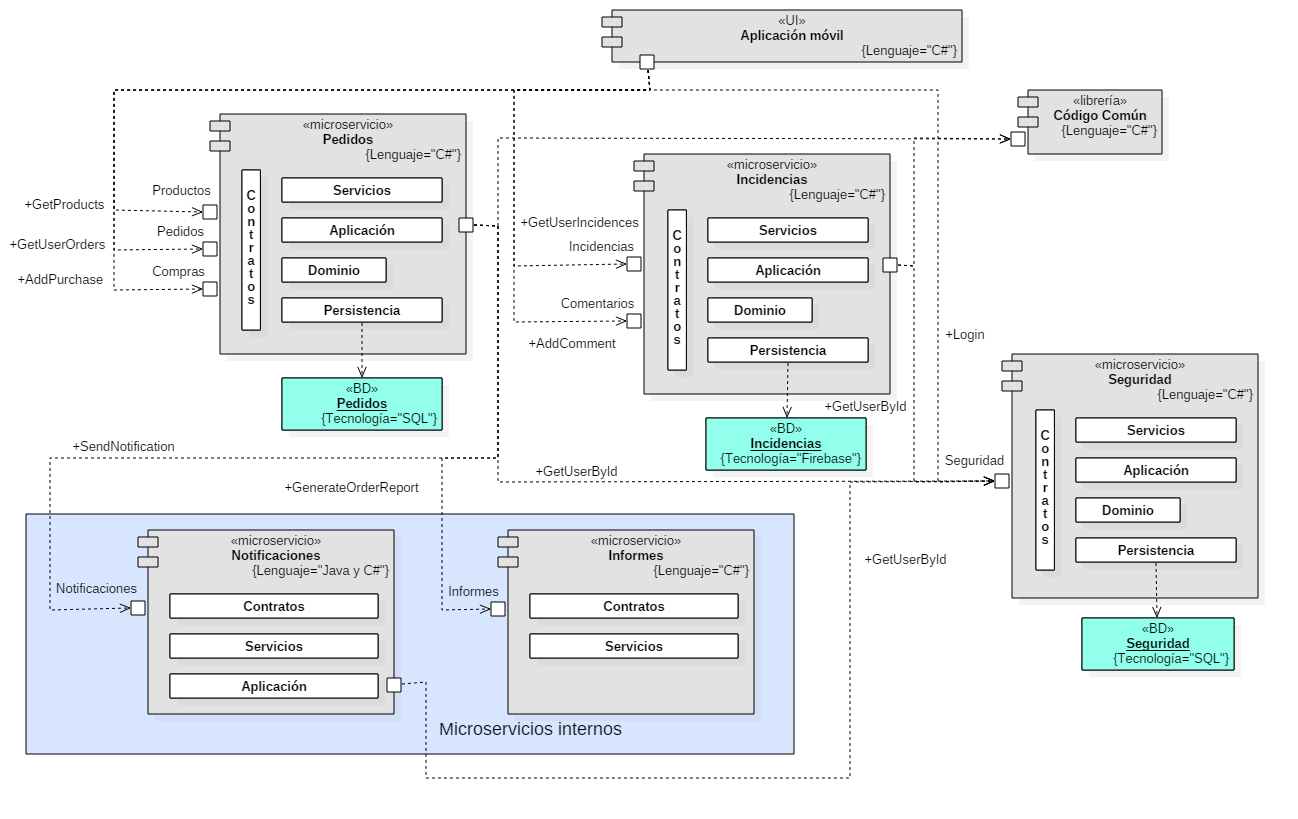
\includegraphics[scale=0.35]{Componentes}
\caption{Diagrama de componentes de la solución basada en microservicios.}
\end{figure}

En la mayoría de microservicios vamos a seguir la arquitectura de 6 capas que se describe en la sección \ref{sct:DiseñoMonolitico} \nameref{sct:DiseñoMonolitico}. Esto hará que su refactorización sea más sencilla ya que sólo debemos copiar las clases relacionadas al microservicio en cada una de las capas. 

Cada microservicio tendrá su propia base de datos, aunque estas pueden localizarse dentro del mismo servidor. Para evaluar otra tecnología de base de datos, la BD del servicio de incidencias la vamos a implementar con Firebase.

Las necesidades de cada microservicio de nuestro caso de estudio son diferentes: algunos como el de informes o notificaciones no requieren persistir datos, por lo que aplicar una arquitectura de 6 capas en ellos no es necesario. 

En el microservicio de informes vamos a seguir una arquitectura más sencilla. Su lógica se situará directamente en la capa de servicios, eliminando la capa de aplicación. Las capas de dominio y persistencia también pueden ser eliminadas porque las plantillas de los informes se van a almacenar como un recurso y no en una base de datos. 

En cuanto al servicio de notificaciones, vamos a implementarlo en el lenguaje Java. Sin embargo, como debe ser consumido por microservicios en lenguaje C\#, construiremos un proxy en este lenguaje para hacer más fácil su consumo.

En el capítulo anterior, en las secciones \ref{subsect:CRUD} \nameref{subsect:CRUD} y \ref{subsect:Persistencia} \nameref{subsect:Persistencia} hemos nombrado algunas interfaces e implementaciones genéricas relacionadas con las entidades de dominio. Los microservicios de pedidos e incidencias deben seguir haciendo uso de estas implementaciones. En el apartado \ref{subsect:librerias} \nameref{subsect:librerias} hemos reflexionado sobre las formas de realizar componentes software. Hacer de este código común un servicio no tiene sentido porque está relacionado con el acceso a datos y cada microservicio es dueño de sus propios datos. En este caso, este código genérico lo referenciarán como una librería a través de paquetes NuGet.

Por último, indicar que el consumo de cualquier microservicio, ya sea desde la interfaz de usuario o desde otros servicios, se realizará a través de las capas de proxy. En el diagrama de componentes no se ha incluido esta capa en la arquitectura interna de ninguno de los microservicios porque esta capa no se ejecuta en el proceso del servicio.

\subsection{Organización de los microservicios}
%Cesar de la Torre.

En cuanto a la organización de los microservicios, vamos a emplear un único repositorio de código que contenga el código de todos los microservicios. Como en la solución monolítica, cada capa se representará a través de un proyecto .NET y cada microservicio tendrá una solución de VS distinta.

En "Building Microservices", Newman reflexiona sobre esto en relación a las compilaciones de integración continua. Según él, la mejor opción es tener un repositorio y una compilación diferente para cada microservicio. De esta forma, existe una mayor correspondencia entre los servicios y los equipos encargados de cada uno porque cada equipo realiza cambios en un único repositorio. Además, se evita que un simple cambio en un microservicio lance la compilación de toda la solución. \cite{Newman2013a} En nuestro caso, no vamos a aplicar las prácticas de integración continua y tampoco tenemos equipos de trabajo distintos, por lo que será más cómodo emplear un único repositorio. Como consecuencia, esto implica que en un mismo commit (la unidad de los repositorios de código git que representa los cambios que se guardan en el repositorio) se puedan incluir cambios de diferentes microservicios.

En cuanto a la organización en soluciones en Visual Studio, en "Microservicios .NET: Arquitectura para Aplicaciones .NET Contenerizadas" se organiza el código de la aplicación desarrollada en un único repositorio con una única solución. \cite{DelaTorre2018} Creemos que esta aproximación no es la mejor. Si consideramos una solución de Visual Studio como una vista de un repositorio de código, no tiene sentido que un desarrollador que trabaja en un único repositorio vea en su solución otros microservicios distintos al suyo. Además, incluir tantos archivos en la solución aumenta su tiempo de compilación, cuando jamás se van a realizar cambios o ejecutar algunos de ellos. Por ello, hemos optado por una solución diferente para cada servicio.

\begin{figure}[h]
\centering
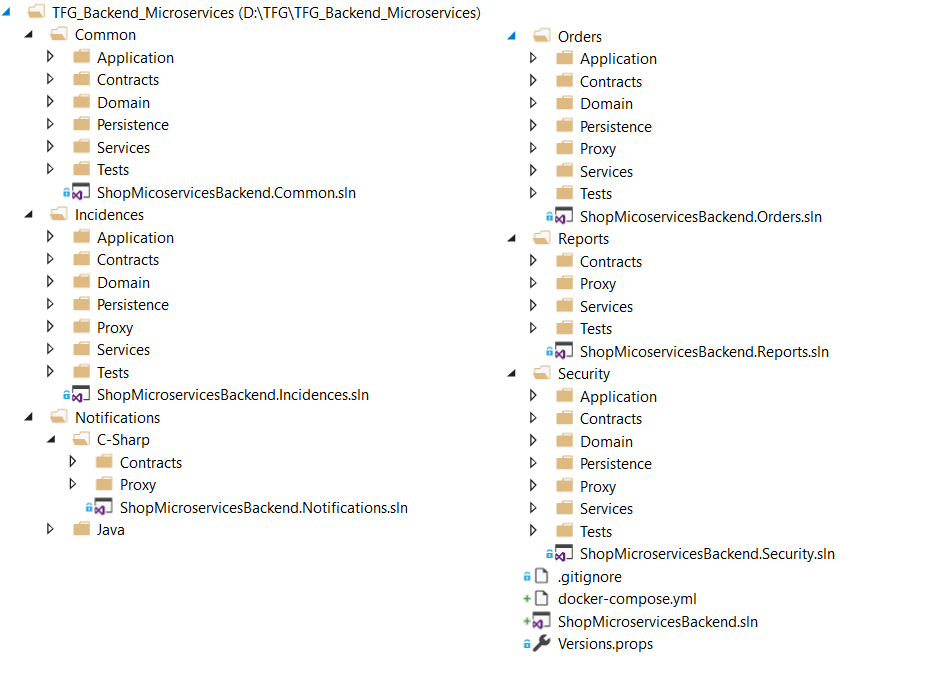
\includegraphics[scale=0.85]{MicroservicesSolution}
\caption{Organización de la solución basada en microservicios.}
\end{figure}

\section{Diferencias en la implementación respecto a la solución monolítica}

\subsection{Consumo de otros microservicios} \label{subsect:Consumo}

Para que un microservicio pueda hacer peticiones a otro se deben seguir los siguientes pasos:

\begin{enumerate}

\item Instalar el paquete NuGet del microservicio a consumir en la capa de aplicación.

\begin{figure}[h]
\centering
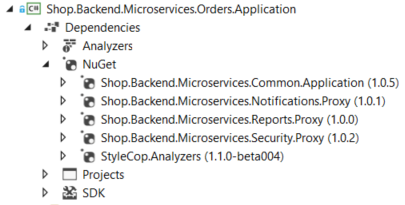
\includegraphics[scale=0.85]{OrdersApplicationDependencies}
\caption{Dependencias del microservicio de pedidos en la capa de aplicación.}
\end{figure}

\item Al registrar las dependencias de la capa de aplicación, invocar al código de la capa de proxy donde se registran las interfaces del microservicio a consumir. En la capa de proxy, las interfaces de la capa de contratos se resuelven con un proxy. Esto significa que en un microservicio cuando hagamos una petición a otro servicio a través de la interfaz se realizará una llamada HTTP a través de su proxy.

\begin{figure}[h]
\centering
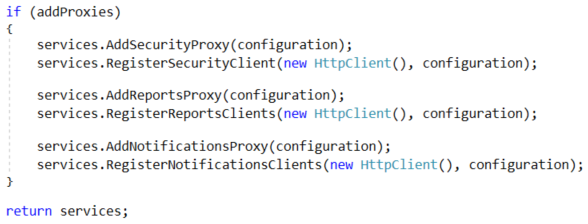
\includegraphics[scale=0.85]{UsingMicroservices}
\caption{Código para resolver otros microservicios consumidos.}
\end{figure}

\item En el microservicio, inyectar en el constructor la interfaz de contratos del servicio que se desea consumir.

\end{enumerate}

%%%%%%%%%%%%%%%%%%%%%%%%%%%
% SALTO DE PAGINA
%%%%%%%%%%%%%%%%%%%%%%%%%%%
\newpage

\subsection{Microservicio de notificaciones}

El microservicio de notificaciones ahora está desarrollado en dos lenguajes de programación distintos: Java y C\#:

En C\# está desarrollado todo lo necesario para el consumo del servicio. Esto incluye la capa de contratos (donde se define su interfaz y el DTO que se empleará en la parte C\#) y la de proxy (donde se indica que la interfaz de contratos se resuelve a través del proxy, que recurre al cliente HTTP para realizar peticiones al microservicio).

\subsection{Consistencia eventual}
%TODO Escribir cambios en la capa de dominio

\begin{figure}[h]
\centering
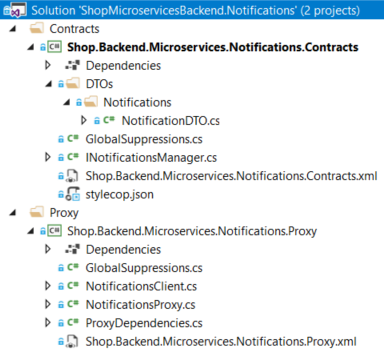
\includegraphics[scale=0.85]{NotificationsC}
\caption{Parte del microservicio de notificaciones desarrollada en C\#.}
\end{figure}

En Java se han desarrollado la capa de aplicación y servicios. La implementación de la capa de aplicación para mandar un correo electrónico es trivial. Para la capa de servicios, se crea e inicia un objeto HttpServer al que se le asigna un handler.

\begin{figure}[h]
\centering
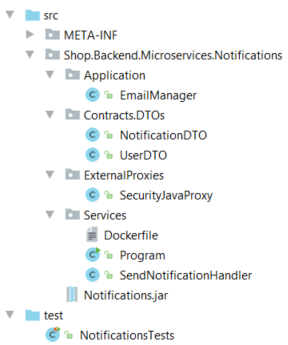
\includegraphics[scale=0.85]{NotificationsJava}
\caption{Parte del microservicio de notificaciones desarrollada en Java.}
\end{figure}

El handler es similar a lo que en .NET llamábamos controlador. En nuestro caso, deserializará el cuerpo (body) de la petición en un objeto empleando la librería Gson y delegará en la capa de aplicación la operación a realizar. Cuando se quiere consumir otro microservicio no podemos emplear los proxies que hemos creado para C\# porque es otro lenguaje de programación. En nuestro ejemplo, queremos contactar con el servicio de seguridad para obtener el correo electrónico de un usuario. Debemos crear un objeto para conectar a través del protocolo HTTP con el microservicio de seguridad y leer la respuesta obtenida.

\begin{figure}[h]
\centering
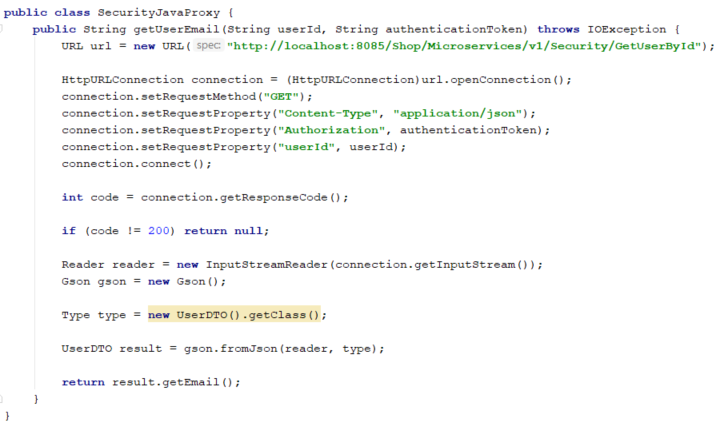
\includegraphics[scale=0.85]{JavaProxy}
\caption{Proxy del microservicio de seguridad para su consumo en Java.}
\end{figure}

Por último, el archivo Dockerfile para el despliegue del servicio también varía. Vamos a seguir el mismo criterio que en los contenedores de microservicios .NET de usar los ensamblados (en este caso, un archivo *.jar) para generar la imagen con el menor número de recursos posibles. Tanto el comando para iniciar el proceso del contenedor como la imagen base se verán afectados.

\begin{figure}[h]
\centering
\includegraphics[scale=1]{JavaDockerfile}
\caption{Dockerfile del microservicio de notificaciones.}
\end{figure}

\subsection{Persistencia en microservicio de incidencias}

En el microservicio de incidencias vamos a emplear una base de datos en la plataforma Firebase. \textbf{Firebase} es una plataforma para el desarrollo de aplicaciones. Uno de los servicios que ofrece es una base de datos NoSQL en la nube en tiempo real. Los datos se almacenan en formato JSON y su acceso puede realizarse a través de peticiones HTTP. \footnote{ Documentación de Firebase Realtime Database: https://firebase.google.com/docs/database/} 

Una de las principales ventajas de las bases de datos NoSQL es su escalabilidad horizontal. En lugar de tener un gran servidor para alojar una base de datos relacional, una base de datos NoSQL se puede distribuir entre diferentes máquinas. Esta funcionalidad en Firebase es de pago, por lo que no vamos a obtener grandes beneficios por emplear esta BD. Nuestro objetivo simplemente es validar que diferentes microservicios pueden emplear tecnologías de bases de datos distintas.

%%%%%%%%%%%%%%%%%%%%%%%%%%%
% SALTO DE PAGINA
%%%%%%%%%%%%%%%%%%%%%%%%%%%
\newpage

\begin{figure}[h]
\centering
\includegraphics[scale=0.85]{Firebase}
\caption{Base de datos de incidencias en Firebase.}
\end{figure}

Gracias a la arquitectura interna basada en capas, el uso de esta BD solo implica dejar de usar la implementación que se da por defecto al DAO en la librería común y programar una implementación propia que acceda a los datos a través de llamadas HTTP.

\begin{figure}[h]
\centering
\includegraphics[scale=0.8]{IncidencesDAO}
\caption{Fragmento de DAO que accede a una base de datos de Firebase.}
\end{figure}

%%%%%%%%%%%%%%%%%%%%%%%%%%%
% SALTO DE PAGINA
%%%%%%%%%%%%%%%%%%%%%%%%%%%
\newpage

\section{Versionado de servicios}
% https://www.thomaslevesque.com/2017/09/18/common-msbuild-properties-and-items-with-directory-build-props/

Cada uno de los microservicios se va a desplegar de forma independiente. El consumo de un microservicio se realiza a través de su proxy, que es una implementación de una interfaz de la capa de contratos. Cuando se realiza y se despliega un cambio en un servicio pueden ocurrir dos situaciones respecto a sus consumidores:

\begin{itemize}

\item  La primera situación es que el cambio \textbf{no haya supuesto un cambio en la interfaz} de la capa de contratos. En este caso, se habrá realizado un cambio a nivel de la lógica del servicio o su persistencia, como puede ser la corrección de un defecto. El cambio realizado no necesita ser conocido por sus consumidores porque están desacoplados de la implementación específica del servicio. 

Los consumidores pueden seguir consumiendo la misma interfaz del servicio. Solo en caso de que se haya modificado el comportamiento del servicio (su especificación) los consumidores deberán ser notificados para adaptarse a cambios en las respuestas del servidor. Por ejemplo, se puede haber cambiado la política de permisos de un método sin haber cambiado su interfaz y ahora devuelve un error 401:Unauthorized porque es necesario otro rol para invocarlo.

\item Una segunda situación consiste en que el cambio \textbf{haya significado un cambio en la interfaz} de contratos. Por ejemplo, puede ocurrir que se haya añadido un nuevo parámetro a un método o se haya cambiado el DTO de respuesta de un método. En este caso, los consumidores deben actualizar el proxy que emplean para comunicar con la nueva versión del servicio. Para asegurar que ningún consumidor se rompe por la actualización se pueden seguir dos aproximaciones según la literatura:

%TODO Esto está muy relacionado con los despliegues V-A y canary releases.
\begin{itemize}

\item \textbf{Mantener la vieja interfaz y redireccionar internamente las peticiones que recibe a la nueva interfaz.} Ambas interfaces están disponibles hasta asegurarse de que ningún cliente esta empleando la interfaz vieja, lo que requiere de la monitorización del servicio para saber cuántos clientes la emplean todavía.

\item \textbf{Tener diferentes versiones del servicio en funcionamiento.} Las peticiones realizadas a la interfaz antigua se redireccionan a la versión vieja del servicio y al contrario con las nuevas peticiones.

Sin embargo, esta aproximación cuenta con algunas desventajas. En primer lugar, si se debe hacer una modificación como solucionar un defecto, posiblemente se deba hacer y desplegar en ambas versiones del servicio. En segundo lugar, se necesita un middleware con la lógica para redireccionar las peticiones a una u otra versión. En conclusión, esta solución puede resultar apta para periodos cortos de tiempo, pero cuanto más tiempo permanezcan los clientes empleando la vieja versión del servicio más riesgo tendremos de que ocurran estos problemas. \cite{Newman2015a}

\end{itemize}

\end{itemize}

En nuestro caso de estudio, tenemos control de todos los consumidores ya que la interfaz de los servicios no va a ser publicada para su consumo por aplicaciones de terceros. Los consumidores de un microservicio serán o la interfaz de usuario u otros servicios. Como hemos comentado en la sección \ref{subsect:Consumo} \nameref{subsect:Consumo}, el proxy se añade como un paquete NuGet con una versión específica. Para asegurarnos de que siempre se consume la última versión de un servicio, vamos a hacer uso de variables para referir a la versión del paquete NuGet a instalar, como se puede ver en la figura \ref{fig:Csproj}.

\begin{figure}[h]
\centering
\includegraphics[scale=0.9]{OrdersNuGets}
\caption{Fragmento del proyecto (.csproj) del servicio de pedidos.}
\label{fig:Csproj}
\end{figure}

A estas variables se les da valor en un archivo llamado Versions.props. Este archivo está centralizado y es común para todos los servicios para que todos ellos referencien a la misma versión de otro microservicio. \footnote{ Common MSBuild properties and items with Directory.Build.props: https://www.thomaslevesque.com/2017/09/18/common-msbuild-properties-and-items-with-directory-build-props/} Cuando se realice un cambio que cambie la interfaz de un servicio, la versión de este se incrementará en una unidad. Los consumidores deberán ser modificados para adaptarse al cambio de la interfaz y deberán desplegarse también. Como se puede ver en el archivo, la versión de cada servicio evoluciona de forma separada.

\begin{figure}[h]
\centering
\includegraphics[scale=0.9]{Versionsprops}
\caption{Archivo Versions.props con las versiones de los microservicios.}
\end{figure}

\section{Adaptación de la interfaz de usuario}

Para que la UI emplee los microservicios que se han creado se debe sustituir el proxy monolítico por los proxies de los microservicios de Seguridad, Incidencias y Pedidos. Esto se hace eliminando el paquete NuGet del proxy monolítico e instalando los tres paquetes nuevos.

Una vez hecho esto, habrá que corregir las referencias a diferentes espacios de nombres. Los espacios de nombre de la solución monolítica a la solución basada en microservicios se han modificado para distinguir clases de ambas soluciones que se llaman igual. Otro cambio que se debe realizar, como muestra la figura \ref{fig:ChangesUI} es invocar el código para resolver las interfaces de contratos con los proxies.

\begin{figure}[h]
\centering
\includegraphics[scale=0.9]{ChangesUI}
\caption{Cambios en la UI para emplear la solución basada en microservicios.}
\label{fig:ChangesUI}
\end{figure}

%TODO Explicar appsettings

\section{Adaptación de las pruebas}

%TODO A la espera de TestServer.

\section{Despliegue}

%%%%%%%%%%%%%%%%%%%%%%%%%%%%%%%%%%%%%%%%%%%%%%%%%%%%%%%%%%%%%%%%%%%%%%%%%%%%%%%
%                       EVALUACIÓN
%
%%%%%%%%%%%%%%%%%%%%%%%%%%%%%%%%%%%%%%%%%%%%%%%%%%%%%%%%%%%%%%%%%%%%%%%%%%%%%%%

\chapter{Evaluación de las soluciones}

\section{Mantenimiento}

\subsection{Mantenimiento correctivo}

El mantenimiento correctivo consiste en una modificación del producto software una vez se ha entregado para corregir un error detectado. \cite{Bourque2014} En piezas de código muy largas resulta difícil encontrar dónde se encuentra un defecto. Gracias al diseño modular de las arquitecturas orientadas a servicios, un defecto será más fácil de localizar. 

En el caso de estudio, un fallo, por ejemplo, en la creación de un pedido se localizará en el microservicio de pedidos. En la misma solución monolítica, si las responsabilidades de las clases no están bien delimitadas, se deberá buscar entre más código para encontrar el defecto.

Sin embargo, esto no siempre es así: dependerá de la interacción entre los servicios. Si para ofrecer una funcionalidad se encadenan muchas peticiones entre servicios diferentes, entender el flujo de invocaciones será más difícil. La interacción basada en eventos también disminuye la comprensión de las comunicaciones. En consecuencia, el proceso de depuración para detectar un defecto será más costoso. Los tokens de correlación son un mecanismo que pueden facilitar esta tarea. Con ellos, se pasa el mismo identificador en cada invocación que se realiza a otro servicio para obtener trazabilidad. \cite{Baum2016}

Por ejemplo, si se observa un fallo de que no se genera correctamente una factura para un cliente, existirán tres microservicios implicados: los de seguridad, informes y pedidos. Para depurar la funcionalidad hace falta una instancia de cada uno de ellos en ejecución. En cambio, en la solución monolítica basta con instanciar un único servicio, el del monolito completo, y en él todas las llamadas se realizarán en el mismo proceso.

\subsection{Mantenimiento perfectivo}

Según la ISO/IEC 14764, el mantenimiento pefectivo es una modificación de un producto software una vez se ha entregado para proveer mejoras a sus usuarios, mejorar la documentación del programa o atributos del software como el rendimiento o la mantenibilidad. \cite{Bourque2014}

Como hemos comentado en el apartado \ref{subsect:Descomposicion} \nameref{subsect:Descomposicion}, el hecho de que se divida la solución en contextos bien delimitados hará que los nuevos requisitos encajen mejor en uno de 

\subsection{Mantenimiento adaptativo}
%Migrar a una nueva plataforma
El mantenimiento adaptativo se define como la modificación de un producto software tras su entrega para que sea utilizable en un nuevo entorno. \cite{Bourque2014}

\section{Comparación de las soluciones ante RNFs}

\subsection{Disponibilidad}

\subsection{Tolerancia a fallos}

\subsection{Utilización de recursos}

\subsection{Capacidad para ser modificado}

Los microservicios incrementan la facilidad de cambio de un producto software. Los microservicios permiten que un cambio en un único servicio se despliegue de manera independiente, haciendo que los cambios lleguen al cliente final de forma más rápida.

\section{Los microservicios en la interfaz de usuario}

\section{Otros posibles diseños de la solución basada en microservicios}
%Reports y notifications como una librería porque no requieren desplegarse frecuentemente y ahorras en llamadas HTTP.

\section{Ventajas e inconvenientes de los microservicios}

%%%%%%%%%%%%%%%%%%%%%%%%%%%%%%%%%%%%%%%%%%%%%%%%%%%%%%%%%%%%%%%%%%%%%%%%%%%%%%%
%                      CONCLUSIONES                                 %
%%%%%%%%%%%%%%%%%%%%%%%%%%%%%%%%%%%%%%%%%%%%%%%%%%%%%%%%%%%%%%%%%%%%%%%%%%%%%%%

\chapter{Conclusiones}

%%%%%%%%%%%%%%%%%%%%%%%%%%%%%%%%%%%%%%%%%%%%%%%%%%%%%%%%%%%%%%%%%%%%%%%%%%%%%%%
%                     BIBLIOGRAFIA                                 %
%%%%%%%%%%%%%%%%%%%%%%%%%%%%%%%%%%%%%%%%%%%%%%%%%%%%%%%%%%%%%%%%%%%%%%%%%%%%%%%

\bibliography{Bibliografia/library}



%%%%%%%%%%%%%%%%%%%%%%%%%%%%%%%%%%%%%%%%%%%%%%%%%%%%%%%%%%%%%%%%%%%%%%%%%%%%%%%
%                           APENDICES  (Si HAY!)                           %
%%%%%%%%%%%%%%%%%%%%%%%%%%%%%%%%%%%%%%%%%%%%%%%%%%%%%%%%%%%%%%%%%%%%%%%%%%%%%%%

\APPENDIX

%%%%%%%%%%%%%%%%%%%%%%%%%%%%%%%%%%%%%%%%%%%%%%%%%%%%%%%%%%%%%%%%%%%%%%%%%%%%%%%
%                      NAVEGACIÓN   
%
%%%%%%%%%%%%%%%%%%%%%%%%%%%%%%%%%%%%%%%%%%%%%%%%%%%%%%%%%%%%%%%%%%%%%%%%%%%%%%%

\chapter{Descripción del prototipo de IU desarrollado} \label{ch:ModeloNavegacion}

%%%%%%%%%%%%%%%%%%%%%%%%%%%%%%%%%%%%%%%%%%%%%%%%%%%%%%%%%%%%%%%%%%%%%%%%%%%%%%%
%                      DESPLIEGUE  
%
%%%%%%%%%%%%%%%%%%%%%%%%%%%%%%%%%%%%%%%%%%%%%%%%%%%%%%%%%%%%%%%%%%%%%%%%%%%%%%%
\chapter{Despliegue del sistema basado en microservicios}

\section{Ejecución de un contenedor con Docker}

\subsection{Archivo Docker Compose}

\section{Introducción a Azure Kubernetes Service (AKS)}

\section{Depuración de contenedores a través de Azure}
% https://blogs.msdn.microsoft.com/benjaminperkins/2017/06/06/remote-debug-your-azure-app-service-2017-including-asp-net-core/ 

\end{document}
